\documentclass[12pt]{article}
\usepackage[utf8]{inputenc}
\usepackage[margin=2.5cm]{geometry}
\usepackage{graphicx}
\usepackage{titlesec}
\usepackage{helvet}
\usepackage[hidelinks,hypertexnames=false]{hyperref}
\usepackage{tocloft}
\usepackage{tabularx}
\usepackage{longtable}
\usepackage{booktabs,array,xltabular,needspace}
\usepackage[section]{placeins}
\usepackage{microtype}
\newcommand{\fuente}[2]{\href{#1}{\textcolor{tpazul}{#2}}}
\raggedbottom
\renewcommand{\topfraction}{0.95}
\renewcommand{\bottomfraction}{0.85}
\renewcommand{\textfraction}{0.05}
\renewcommand{\floatpagefraction}{0.8}
\setcounter{topnumber}{4}
\setcounter{totalnumber}{5}
\makeatletter
\setlength{\@fptop}{0pt}
\makeatother
\setlength{\emergencystretch}{2em}
\widowpenalty=10000
\clubpenalty=10000
\IfFileExists{spanish.ldf}{\usepackage[spanish]{babel}}{%
  \usepackage{babel}\babelprovide[import,main]{spanish}}

\usepackage{xcolor}
\usepackage{tikz}
\usepackage{float}
\usetikzlibrary{arrows.meta,calc,fit,backgrounds,babel}
\definecolor{tpazul}{HTML}{1F4E79}
\definecolor{tpclaro}{HTML}{EAF2F8}
\definecolor{tpverde}{HTML}{E2F0D9}
\definecolor{tpenergia}{HTML}{FCE4D6}
\newcommand{\consigna}{\color{green!50!black}\itshape}
\renewcommand{\familydefault}{\sfdefault}

% INICIO SUBSUBSUB
%same as \subsubsection but level 4
\makeatletter
\renewcommand\paragraph{\@startsection{paragraph}{4}{\z@}%
                                     {-3.25ex\@plus -1ex \@minus -.2ex}%
                                     {1.5ex \@plus .2ex}%
                                     {\normalfont\normalsize\bfseries}}
% number \paragraph
\setcounter{secnumdepth}{4}
\makeatother
% FIN SUBSUBSUB

\usepackage{draftwatermark}

\tikzset{
        bloque/.style={draw=tpazul!65,fill=tpclaro,rounded corners=3pt,
            text width=2.5cm,minimum height=1.15cm,inner sep=5pt,
            align=center,font=\sffamily\footnotesize},
        sensor/.style={bloque,fill=tpverde},
        energia/.style={bloque,fill=tpenergia},
        externo/.style={bloque,fill=white,draw=tpazul!40},
        flujo/.style={-{Stealth[length=2mm]},line width=.8pt,draw=tpazul},
        potencia/.style={flujo,dashed,draw=orange!70!black},
        relacion/.style={line width=.8pt,draw=tpazul},
        rotulo/.style={font=\sffamily\scriptsize,fill=white,inner sep=2pt,text=tpazul},
        marco/.style={draw=tpazul!35,rounded corners=5pt,fill=black!1,inner sep=12pt},
        titulo/.style={font=\sffamily\bfseries\large,text=tpazul,anchor=west}
    }
    
\AddToHook{cmd/section/before}{\par\Needspace{7\baselineskip}}
\AddToHook{cmd/subsection/before}{\par\Needspace{5\baselineskip}}
\AddToHook{cmd/subsubsection/before}{\par\Needspace{5\baselineskip}}
\AddToHook{cmd/paragraph/before}{\par\Needspace{4\baselineskip}}
\begin{document}
% Marca de agua
\SetWatermarkText{}
\SetWatermarkScale{0.4}
\SetWatermarkLightness{0.8}
\SetWatermarkAngle{45}
\SetWatermarkColor{red!20!white}
% Fin - Marca de agua

% Portada
\begin{titlepage}
    \centering
    
\includegraphics[width=0.6\textwidth]{logo-fiuba.png} \\
    \vspace{2cm}
    {\Huge Sistema Inteligente Multimodal de Detección y Predicción de Glucosa} \\
    \vspace{0.5cm}
    {\LARGE Materia: TC024 - Gestión de proyectos} \\
    \vspace{2cm}
    \begin{flushleft}
        \textbf{Título del trabajo final:} Sistema Inteligente Multimodal de Detección y Predicción de Glucosa\\
        \vspace{2cm}
        \noindent\makebox[\linewidth]{\rule{\textwidth}{0.4pt}}\\[0.5cm]
        \begin{tabularx}{\textwidth}{XXX}
            \textbf{Autor:} & \textbf{Padrón:} & \textbf{Correo:} \\
            Marco Brischetto & 110008 & mbrischetto@fi.uba.ar \\
            Lautaro García Vitale & 110028 & lagarciav@fi.uba.ar \\
            Gabriel José Vigo Abad & 107980 & gvigo@fi.uba.ar \\
            Juan Ignacio Giachetti & 110877 & jgiachetti@fi.uba.ar \\
            Ignacio E. Cavicchioli & 109428 & icavicchioli@fi.uba.ar \\
            Martina Monti &  110574& mmonti@fi.uba.ar \\
            Francisco Del Rio & 110761 & fadelrio@fi.uba.ar \\
            Santiago Manuel Cabrera & 110445 & smcabrera@fi.uba.ar \\

        \end{tabularx}
    
    \end{flushleft}
    \noindent\makebox[\linewidth]{\rule{\textwidth}{0.4pt}}\\[0.5cm]
    \vfill
    \Large Facultad de Ingeniería - Universidad de Buenos Aires
\end{titlepage}

\setcounter{tocdepth}{4}
\tableofcontents
%****************    INTRODUCCION  **********%
\clearpage
\section{Introducción}
{\consigna
Debe contener una descripción del contexto en el que se ubica el proyecto, su función y el lugar que ocupa.\\
Luego de leer la introducción, el lector debe poder imaginarse de qué se trata el proyecto, sus beneficios, la problemática que aborda o resuelve y la complejidad esperada del mismo.\\
Esta sección sirve como un resumen anticipado oficial del proyecto para que el lector decida si le interesa dedicar tiempo a leer el detalle del proyecto en las siguientes secciones.
}

Las alteraciones de la glucosa requieren seguimiento y pueden generar preocupación e incertidumbre en los pacientes. En los últimos años, los monitores continuos de glucosa (CGM) han incorporado funciones de seguimiento y, en algunos casos, de predicción de su evolución. Aun así, interpretar cómo se relacionan las variaciones observadas con la alimentación, el estrés o la actividad física suele requerir registros adicionales y evaluación profesional.

En este contexto, el proyecto propone desarrollar un sistema portátil e inteligente que integre mediciones de biomarcadores en sudor con señales fisiológicas de contexto para identificar factores probablemente asociados a una variación y explorar dos horizontes de predicción como objetivos de diseño. El análisis se limitará a un conjunto finito y predefinido de factores habituales, como la alimentación, el estrés y la actividad física, organizado en una base de referencia cuya selección y validación formarán parte del desarrollo. Al relacionar las mediciones con esos factores, el sistema buscará ofrecer una explicación contextual de la variación observada, indicando cuando la información disponible no permita distinguir entre ellos. Esta identificación será una asociación estimada, no una determinación de la causa ni una evaluación de todas las causas posibles, y no equivaldrá a establecer causalidad clínica. Las mediciones de glucosa en sudor tampoco se presentarán como mediciones directas de glucosa sanguínea: deberá definirse y validarse la referencia de evaluación de cada salida del sistema.

De esta manera, la solución apunta a complementar a los CGM existentes mediante información contextual y avisos acordes con un uso previsto todavía por definir. La eventual dependencia de datos de un CGM y el modo de integración con esos dispositivos quedan pendientes de decisión. Una mejora del seguimiento cotidiano, del bienestar de los usuarios o del uso de recursos sanitarios constituye un beneficio esperado que deberá evaluarse, no un efecto demostrado.


%****************    DEFINICION DEL PROYECTO  **********%

\section{Definición del proyecto}
{\consigna
Esta sección debe definir el proyecto. A diferencia de la introducción, que es más ``blanda'', a lo largo de esta sección y subsecciones, se debe ser claro y específico, tratando de minimizar posibles ambigüedades.
Si vamos a hacer un sistema compuesto por un microcontrolador, sensores para medir ciertos indicadores, registrarlos y decidir tomar alguna acción en base a esos datos con cierta finalidad, digamos eso mismo: ``un sistema compuesto por un microcontrolador, sensores para medir ciertos indicadores, registrarlos y decidir tomar alguna acción en base a esos datos con'' la finalidad que sea.\\


En esta parte introductoria de la sección, se puede describir el objetivo de negocio que se persigue y cómo se espera cumplirlo, de forma de facilitar el entendimiento de las siguientes subsecciones.
}

El proyecto consiste en el desarrollo de un sistema portátil e inteligente compuesto por dos dispositivos complementarios —un dispositivo no invasivo ubicado en la parte posterior del brazo, formado por un parche sensor descartable y un módulo electrónico reutilizable de lectura y comunicación que se acopla a él, y una pulsera de muñeca reutilizable— junto con una capa de procesamiento e inteligencia artificial, destinado a personas con diabetes tipo 2 y pre-diabetes.

El parche sensor descartable permite medir glucosa, lactato y cortisol en sudor mediante el módulo electrónico reutilizable, mientras que la pulsera capta señales fisiológicas de contexto (frecuencia cardíaca, actividad física y temperatura de piel). El sistema integra ambas fuentes de datos para no solo reportar el nivel de glucosa, sino explicar su causa probable (alimentación, estrés, actividad física o una posible complicación renal) y predecir su evolución en dos modos complementarios: corto plazo (30 a 60 minutos), orientado a priorizar la exactitud de la predicción, y horizonte extendido (1 a 8 horas), orientado a estimar tendencias para apoyar la planificación del seguimiento, entregando al usuario una alerta temprana junto con una recomendación de acción concreta.

El dispositivo busca integrar en una única solución información que hoy se obtiene mediante distintos controles y análisis dispersos en el tiempo, complementando —no reemplazando— a los medidores de glucosa continuos (CGM) existentes en el mercado.


% la V 2.6 se reodena la sección misión y vision antes de Objetivo
\subsection{Misión y visión}
{\consigna
Esta subsección debe definir la Misión y la Visión del proyecto.\\
La **misión** es la razón de ser del proyecto basada en su propósito principal, mientras que la **visión** es la imagen de cómo se espera que el proyecto pueda evolucionar a futuro. La misión se enfoca en el presente y en lo que el resultado del proyecto hace para cumplir su propósito, mientras que la visión se enfoca en el futuro y en los posibles objetivos que el proyecto busca alcanzar.\\
Existe mucho material disponible para ayudar al alumno a definir estas dos características de su proyecto.
}

Desarrollar una solución portátil que integre mediciones no invasivas de biomarcadores en sudor y señales fisiológicas para aportar información contextual e identificar factores probablemente asociados a las variaciones observadas, sin atribuir causalidad clínica, con el propósito de facilitar el seguimiento de la salud metabólica.

A futuro, se busca consolidar una forma de seguimiento de la salud metabólica que combine mediciones, estimaciones e información contextual con evidencia suficiente para orientar su interpretación. En versiones posteriores podría evaluarse la incorporación de funciones relacionadas con complicaciones asociadas a la diabetes, como el daño renal, únicamente si existe evidencia que las sustente y se realiza una validación específica. La eventual contribución a la autonomía y seguridad de los pacientes o a un uso más eficiente de los recursos sanitarios deberá demostrarse mediante evaluaciones apropiadas.


\subsection{Objetivo}
{\consigna
Esta subsección debe definir el objetivo puntual del proyecto, el resultado esperable, de forma más específica que la definición previa, en cuanto a qué esperar. Debe especificarse si se espera un prototipo o un producto final, y con qué calidad. Si el resultado se compone de varias partes, deben especificarse todas.\\
El objetivo aquí descripto debe cumplir con el paradigma S.M.A.R.T. El lector debe entender completamente qué esperar como resultado del proyecto.
}

El objetivo del proyecto es construir un sistema portátil y funcional compuesto por un parche sensor descartable de biomarcadores en sudor, un módulo electrónico reutilizable de lectura y comunicación que se acopla al parche sensor, una pulsera reutilizable de señales fisiológicas y una aplicación móvil, que permita realizar un seguimiento de marcadores biométricos, identificar factores probablemente asociados a las variaciones observadas y estimar la evolución de la glucosa en dos horizontes de predicción: corto plazo (30 a 60 minutos) y horizonte extendido (1 a 8 horas). La identificación de factores se limitará a un conjunto finito y predefinido, como la alimentación, el estrés y la actividad física, sin establecer causalidad clínica. El sistema deberá presentar las mediciones, las estimaciones y los avisos correspondientes para facilitar el seguimiento cotidiano del usuario; el desempeño de sus funciones deberá verificarse mediante pruebas de aceptación.

Como resultado se entregarán cuatro componentes integrados: una aplicación móvil, un parche sensor descartable, un módulo electrónico reutilizable de lectura y comunicación, y una pulsera reutilizable. La aplicación deberá vincularse con el módulo y la pulsera, recibir y presentar sus datos e implementar las funciones de análisis, historial, avisos y ayuda comprometidas para la versión. El parche descartable comprenderá el sustrato de papel, sus zonas con reactivos y el soporte adhesivo; se establece como objetivo reemplazarlo cada 7 días de uso, sujeto a validar la estabilidad de los reactivos, la adhesión y el desempeño. El módulo electrónico reutilizable se acoplará al parche e incluirá los elementos de lectura, procesamiento, comunicación, firmware y alimentación que se definan. La pulsera reutilizable incluirá sus sensores, electrónica, firmware y alimentación. Los tres componentes físicos se entregarán protegidos en un paquete que los identifique e incluya la lista de contenido, los accesorios y consumibles definidos, y las instrucciones de puesta en marcha, conexión con la aplicación, mantenimiento de los elementos reutilizables y recambio del parche. La aplicación móvil no requiere reemplazo físico.

%\noindent\textbf{Pendiente de definir:} el plazo de desarrollo del producto, la cantidad de kits que se producirán, las plataformas compatibles con la aplicación, los umbrales de desempeño para la aceptación y si el resultado será un prototipo funcional de evaluación o un producto final comercial. Estas decisiones no se vinculan con la fecha de entrega de la actividad académica.


\subsection{Entregables mensurables}
{\consigna
Esta subsección debe definir cuáles serán los resultados esperables para verificar el éxito del proyecto.\\
Se debe especificar concretamente cómo el verificador puede constatar, al final del proyecto, que se cumplieron los objetivos del mismo. Esta descripción da certidumbre a la vez que ayuda a especificar mejor los requerimientos del proyecto.
}


Se considerará cumplido el objetivo del proyecto con la entrega y aceptación de los siguientes cuatro componentes:

\begin{enumerate}
    \item \textbf{Aplicación instalable:} deberá permitir la vinculación por BLE con el módulo electrónico reutilizable y la pulsera, la recepción y visualización de datos, la consulta del historial, las funciones de análisis comprometidas para la versión, la presentación de avisos acordes con el uso previsto y el acceso a la ayuda. La aplicación móvil no requiere reemplazo físico. Las estimaciones deberán informar su horizonte temporal y su incertidumbre. La aceptación verificará la instalación, la vinculación, la transmisión, el historial y la respuesta ante fallas; el desempeño de cada modelo se evaluará por separado conforme a los umbrales pendientes de definir.
    \item \textbf{Parche sensor descartable:} parche de papel con sus zonas con reactivos y soporte adhesivo para la medición de los biomarcadores previstos en sudor. El objetivo es reemplazar la parte no reutilizable del parche cada 7 días de uso.
    \item \textbf{Módulo electrónico reutilizable:} módulo acoplable al parche sensor, con lector óptico, front-end electroquímico, microcontrolador, BLE, firmware y alimentación, según el diseño detallado. La aceptación verificará el acoplamiento con el parche, la adquisición y procesamiento de las lecturas, la transmisión de datos a la aplicación, las tolerancias que se definan y una autonomía objetivo de al menos 7 días de uso normal.
    \item \textbf{Pulsera reutilizable:} dispositivo con PPG, sensor de temperatura, IMU, BLE, firmware y alimentación, según el diseño detallado. La aceptación verificará la adquisición y transmisión de las señales previstas, la integración con la aplicación, las tolerancias que se definan y una autonomía objetivo de al menos 7 días de uso normal. 
\end{enumerate}

Los tres componentes físicos se entregarán protegidos en un paquete identificado, con lista de contenido, accesorios y consumibles definidos, guía rápida, manual y guía de solución de problemas. Sus instrucciones deberán cubrir la puesta en marcha, la conexión con la aplicación, el mantenimiento del módulo y la pulsera, y el recambio del parche descartable. El paquete es una condición de presentación y entrega, no un quinto componente del sistema.

%****************    EVALUACION DEL PROYECTO  **********%



\section{Evaluación del proyecto}
{\consigna
Esta sección aborda el análisis del proyecto con el objetivo de evaluarlo desde dos aspectos: **Técnico** y de **Negocio**.\\
En la **evaluación Técnica** se analizan la factibilidad, los riesgos y todas las cuestiones que aborda el proyecto desde lo tecnológico.\\
En la **evaluación de Negocio** se analizan los aspectos relacionados con la receptividad o posibilidades de adopción del resultado del proyecto por parte de los destinatarios del mismo y las posibilidades de realización desde lo organizacional, legal, económico y demás posibles aspectos no tecnológicos que deban considerarse.
}


\subsection{Tipo de proyecto}
{\consigna
Esta subsección aborda la tipificación del proyecto o su encuadre dentro del tipo de despliegue que el resultado del proyecto va a tener.\\
En clase hemos propuesto los siguientes tipos:
\begin{itemize}
\setlength{\itemsep}{0pt}
  \item Proyectos Masivos
  \item Proyectos Específicos
  \item Proyectos Únicos o a Medida
  \item Proyectos de Innovación o Investigación
\end{itemize}
Esta lista es una propuesta y puede ampliarse o incluso definir una tipificación diferente.
}


El proyecto se clasifica como un Proyecto Masivo por el despliegue previsto de un producto estandarizado, fabricable y distribuible de forma repetible a numerosos usuarios. El resultado mantiene un diseño común compuesto por una aplicación, un conjunto sensor ---que integra el parche sensor descartable, el módulo electrónico reutilizable de lectura y comunicación y la pulsera reutilizable--- y el paquete del sensor. El segmento inicial está constituido por personas con diabetes tipo 2 o prediabetes; la definición de este público no convierte al proyecto en una solución a medida de un único comprador. La configuración individual de parámetros de uso o seguimiento tampoco modifica el diseño común del producto.

Este enfoque exige definir criterios que favorezcan la consistencia entre unidades, una instalación y puesta en marcha comprensibles, la provisión y el recambio de consumibles, el soporte a los usuarios y el análisis de los costos por unidad. Se trata de condiciones a considerar durante el desarrollo: la clasificación no implica que se hayan alcanzado determinados volúmenes o niveles de adopción, ni demuestra por sí misma la factibilidad técnica, la validación del desempeño, la habilitación regulatoria o la madurez comercial del producto.


\subsection{Evaluación de factibilidad técnica}
{\consigna
Esta subsección aborda la evaluación Técnica para analizar la factibilidad, los riesgos y todas las cuestiones que involucran el proyecto desde lo tecnológico.\\
En las diferentes subsecciones se pretenden cubrir todos los aspectos técnicos de la evaluación.
}

Esta sección evalúa la factibilidad técnica del sistema propuesto. Varios de los principios de sensado utilizados —en particular el sensado simultáneo de múltiples biomarcadores en un mismo dispositivo— provienen de desarrollos recientes documentados en literatura científica; el proyecto los adopta y adapta al caso de uso de diabetes, sin que esto implique que la generación de ese conocimiento sea en sí misma el objetivo del trabajo.

\subsubsection{Requerimientos técnicos}
{\consigna
En este apartado deben definirse todos los requerimientos técnicos que deberá cumplir el proyecto, que serán la especificación para el diseño de la solución a construir.\\
Debe contemplar los requisitos que, de cumplirse, cubren las expectativas del proyecto.\\
Todo lo que no se mencione puede no estar y aun así el proyecto ser exitoso.\\
Estas especificaciones suelen usarse durante la verificación para evaluar el cumplimiento del objetivo.\\
Los requerimientos técnicos incluyen los tecnológicos y los funcionales.
}

\noindent\textbf{Requerimientos funcionales:}
\begin{enumerate}
    \item Medir glucosa, lactato, cortisol y pH en sudor de forma no invasiva mediante el parche sensor descartable y el módulo electrónico reutilizable de lectura y comunicación. El pH se utilizará como referencia para la calibración de las demás zonas. Estas mediciones deberán distinguirse de cualquier estimación de glucosa sanguínea.
    \item Medir frecuencia cardíaca, actividad física y temperatura de piel mediante la pulsera, como contexto fisiológico.
    \item Evaluar por separado dos modos propuestos como objetivos de diseño para estimar la evolución de la glucosa: corto plazo (30 a 60 minutos) y horizonte extendido (1 a 8 horas). En ambos modos se deberá indicar el horizonte temporal y la incertidumbre, sin presuponer su viabilidad ni un nivel de precisión ya alcanzado.
    \item Identificar factores probablemente asociados a una variación (alimentación, estrés o actividad física), aclarando que el resultado no establece causalidad clínica.
    \item Presentar información y avisos al usuario acordes con el uso previsto, todavía pendiente de definir, sin emitir recomendaciones automáticas de tratamiento.
    \item Transmitir los datos del módulo electrónico reutilizable y de la pulsera al teléfono por BLE, con una sincronización nominal cada 5 minutos, ajustable según la experiencia de uso. Este intervalo corresponde a la transferencia y no fija la frecuencia de muestreo. Ante una pérdida del enlace, conservar localmente en cada dispositivo al menos 24 horas de datos (estimación: 45 KiB por día y por dispositivo) y transmitir el bloque acumulado al restablecerse BLE.
    \item Definir, antes de evaluar el desempeño, la referencia correspondiente a cada salida, incluidas las mediciones en sudor y cualquier estimación de glucosa sanguínea.
    \item Mantener la solución como complemento de los CGM y documentar como decisión pendiente si los modelos dependerán de datos de un CGM y cómo se realizaría esa integración.
\end{enumerate}

\noindent\textbf{Requerimientos técnicos}
\par\medskip
{\small
\renewcommand{\arraystretch}{1.2}
\begin{xltabular}{\textwidth}{|>{\raggedright\arraybackslash}p{0.28\textwidth}|>{\raggedright\arraybackslash}X|}
\hline
\textbf{Componente} & \textbf{Requerimiento} \\
\hline
\endfirsthead
\hline
\textbf{Componente} & \textbf{Requerimiento} \\
\hline
\endhead
Zona glucosa (parche sensor descartable) & Colorimétrica --- reactivo cromogénico específico \\
\hline
Zona lactato (parche sensor descartable) & Colorimétrica --- reactivo cromogénico específico \\
\hline
Zona pH (parche sensor descartable) & Colorimétrica --- referencia/calibración de las demás zonas \\
\hline
Zona cortisol (parche sensor descartable) & Electroquímica --- polímero de impronta molecular (MIP) \\
\hline
Parche sensor descartable & Papel tratado hidrofílica/hidrofóbicamente, plegado tipo origami (microfluídica de papel, bajo costo), incluidas sus zonas con reactivos y su soporte adhesivo. Objetivo de recambio del parche sensor completo cada 7 días de uso, sujeto a validar estabilidad de reactivos, adhesión y desempeño \\
\hline
Lector óptico & Sensor de color para las zonas colorimétricas del parche sensor descartable, integrado en el módulo electrónico reutilizable \\
\hline
Front-end electroquímico & Circuito simple de un solo canal (potenciostato) dedicado a la zona de cortisol, integrado en el módulo electrónico reutilizable \\
\hline
Sensor óptico (pulsera) & PPG para frecuencia cardíaca, idealmente integrado con sensor de temperatura de piel en el mismo IC; pulsera y electrónica reutilizables \\
\hline
IMU (pulsera) & Acelerómetro + giróscopo para detección de actividad/movimiento \\
\hline
Microcontrolador & Bajo consumo, procesa lecturas ópticas y electroquímicas, calibración adaptativa; integrado en el módulo electrónico reutilizable \\
\hline
Comunicación & BLE en el módulo electrónico reutilizable y la pulsera; sincronización nominal cada 5 minutos, ajustable según experiencia de usuario; alcance objetivo de hasta 10 m, incluyendo uso del teléfono en el bolsillo, a validar en pruebas típicas \\
\hline
Almacenamiento local y sincronización & Buffer de al menos 24 horas por dispositivo (estimación: 45 KiB/día). Sincronización cada 5 minutos si BLE está disponible; al reconectar, envío en bloque de los datos acumulados. Para interrupciones superiores a 24 horas no se garantiza conservar el excedente; la aplicación deberá señalar los intervalos faltantes. Validar capacidad y retención ante apagado. \\
\hline
Procesamiento de IA & Modelos a evaluar por separado: estimación temporal (30 a 60 minutos y 1 a 8 horas) e identificación de factores probablemente asociados, sin causalidad clínica. Ejecución local en el teléfono o remota en la nube, coordinada por la aplicación; selección pendiente según costos y requisitos de funcionamiento. La aplicación móvil no requiere reemplazo físico \\
\hline
Alimentación & Batería recargable de bajo consumo en el módulo electrónico reutilizable y en la pulsera reutilizable; autonomía objetivo de al menos 7 días de uso normal para ambos, con perfil de muestreo por definir y a validar \\
\hline
\end{xltabular}
\par}


\subsubsection{Diseño preliminar del producto}
{\consigna
En este apartado debe ir completándose el diseño preliminar. Es un primer bosquejo de diseño que permite tomar dimensión del proyecto y una primera propuesta a alto nivel de solución para cumplir el objetivo y atender los requerimientos.\\
Esta sección lleva más tiempo completarla porque implica la elaboración de un diseño de circuito, sistema, partes, etc.\\
Puede contener diagramas en bloque, especificación de partes y demás detalles que den certidumbre sobre la posibilidad de realización. No es necesario que tenga todo el detalle tecnológico.
}

El sistema se organiza en dos fuentes de datos que convergen en una aplicación central (app/hub), como se muestra en la Figura~\ref{fig:arquitectura-sistema}. El dispositivo del brazo está formado por un parche sensor descartable, ubicado en la parte posterior del brazo, y un módulo electrónico reutilizable de lectura y comunicación que se acopla a él. El parche sensor consiste en papel tratado hidrofílica/hidrofóbicamente y plegado tipo origami, con sus zonas con reactivos y su soporte adhesivo. Sus zonas colorimétricas permiten medir glucosa, lactato y pH en sudor mediante reactivos cromogénicos y un sensor de color situado en el módulo electrónico reutilizable; la zona de pH se utiliza como referencia para la calibración de las demás zonas. Una zona electroquímica separada del parche sensor, basada en un polímero de impronta molecular (MIP), permite medir cortisol en sudor mediante un potenciostato de un solo canal integrado en el módulo electrónico reutilizable. Estas mediciones no constituyen por sí mismas mediciones de glucosa sanguínea: cualquier salida que la estime deberá especificar su referencia de evaluación. La pulsera reutilizable, en la muñeca, integra el sensor óptico PPG, el sensor de temperatura, la IMU y su propio módulo BLE, todos reutilizables, aportando el contexto fisiológico de frecuencia cardíaca, actividad física y temperatura de piel. El módulo electrónico reutilizable y la pulsera transmiten sus datos por BLE a la aplicación central (hub), donde se proponen modelos de inteligencia artificial que deberán evaluarse por separado: un modelo temporal con objetivos de diseño de corto plazo (30 a 60 minutos) y horizonte extendido (1 a 8 horas), sin presuponer la viabilidad ni la precisión de ninguno de ellos; y un modelo que identifica factores probablemente asociados a la variación al relacionar biomarcadores y señales fisiológicas de contexto, sin establecer causalidad clínica. Cada salida deberá presentar su horizonte temporal, incertidumbre y referencia de evaluación según corresponda. La aplicación presentará información y avisos coherentes con el uso previsto, aún pendiente de cerrar, sin recomendaciones automáticas de tratamiento. El sistema se concibe como complemento de los CGM; queda pendiente determinar si los modelos dependerán de sus datos y cómo se integrarían.

La aplicación central se ejecutará en el teléfono del usuario y recibirá los datos del módulo electrónico reutilizable y la pulsera. Para ejecutar los modelos de IA se evaluarán dos alternativas: procesamiento local\footnote{El modelo local que se ejecutaría es el que proyecta los datos a futuro, no es un modelo de lenguaje.} en el teléfono o procesamiento remoto en un servicio en la nube, al que la aplicación enviaría los datos necesarios y del que recibiría los resultados. La elección se realizará durante el diseño detallado, comparando los costos de implementación y operación, la capacidad de procesamiento del teléfono, el tiempo de respuesta, la disponibilidad de conexión a Internet y los requisitos de privacidad y protección de datos. No se compromete en esta etapa la implementación de ambas modalidades. Si se elige la nube, deberá definirse el comportamiento del sistema ante la pérdida de conexión, indicando al usuario qué funciones no estarán disponibles.

La comunicación entre el módulo electrónico reutilizable, la pulsera y el teléfono tendrá un intervalo nominal de sincronización de 5 minutos, ajustable según la experiencia de uso. Se buscará un alcance BLE que cubra el uso del teléfono en el bolsillo y hasta 10 m en condiciones típicas; ambos aspectos deberán validarse en pruebas. Este intervalo es de transferencia y no define la frecuencia de muestreo. Si el teléfono se aleja o se apaga mientras el módulo y la pulsera siguen encendidos, estos conservarán localmente hasta 24 horas de datos cada uno (estimación: 45 KiB por día y dispositivo) y enviarán el bloque acumulado al restablecerse BLE. Si la interrupción supera las 24 horas, no se garantiza conservar el excedente y la aplicación deberá indicar los intervalos faltantes, sin presentar la serie como continua. Si los propios dispositivos se apagan, no se adquieren mediciones durante ese período; la persistencia de los datos ya almacenados ante un apagado dependerá de la memoria elegida y deberá verificarse. La estimación de memoria se considera compatible con microcontroladores habituales, sujeta a validación con el formato, las marcas temporales, los metadatos y las frecuencias de muestreo definidos.

El consumible descartable del sistema será el parche sensor de papel completo, incluidas sus zonas con reactivos y su soporte adhesivo de fijación a la piel del brazo. Se establece como objetivo reemplazar el parche sensor completo cada 7 días de uso, sujeto a validar la estabilidad de los reactivos, la adhesión y el desempeño, conservando el módulo electrónico reutilizable de lectura y comunicación que se acopla a él. La pulsera y su electrónica también serán reutilizables. La aplicación móvil no requiere reemplazo físico. La vida útil objetivo de 7 días y las instrucciones para retirar, reemplazar y volver a acoplar el parche sensor deberán validarse durante el desarrollo.

El diseño preliminar se presenta mediante diagramas por objeto.
La Figura~\ref{fig:parche-descartable} muestra el parche sensor
 descartable; la Figura~\ref{fig:lector-reutilizable}, el lector
reutilizable del brazo; la Figura~\ref{fig:pulsera-reutilizable},
la pulsera; la Figura~\ref{fig:aplicacion-movil}, la aplicación
móvil; y la Figura~\ref{fig:caja-producto}, el paquete del sensor.
La Figura~\ref{fig:arquitectura-sistema} resume el flujo de datos y las dos alternativas de procesamiento. Las líneas discontinuas indican el procesamiento remoto: la aplicación intercambia los datos necesarios y los resultados con la nube mediante Internet (Wi-Fi o datos móviles); los dispositivos se comunican únicamente con el teléfono por BLE. Si se elige IA local, el procesamiento se realiza en el teléfono.



\begin{figure}[H]
    \centering
    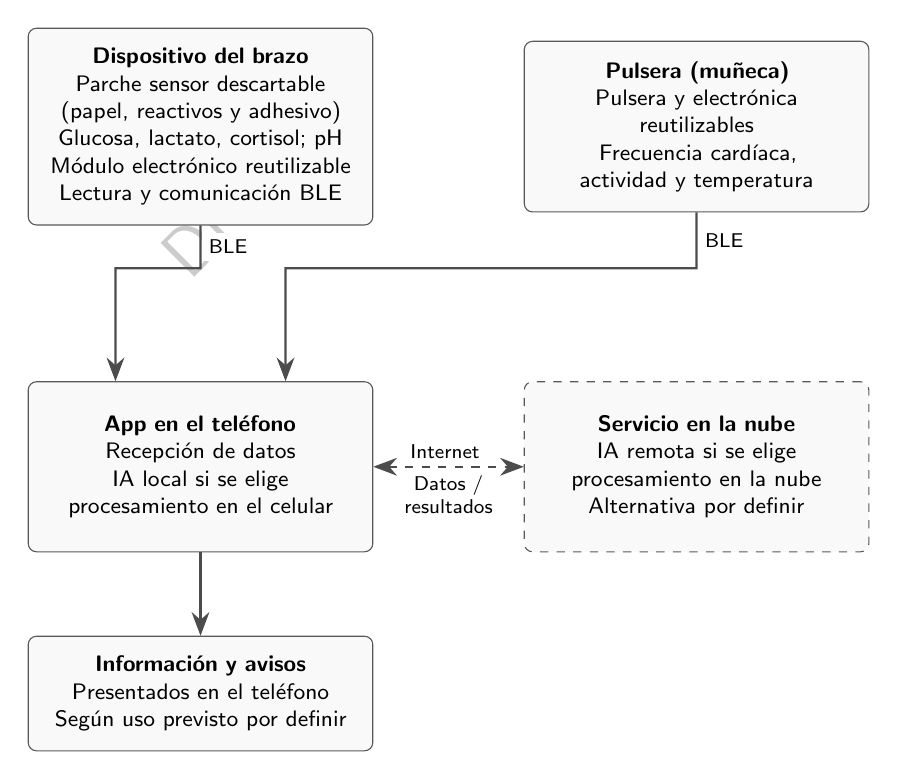
\begin{tikzpicture}[scale=0.9,transform shape,
        bloque/.style={draw=black!65, rounded corners=3pt, fill=gray!5,
            align=center, font=\small, text width=4.3cm,
            minimum height=2.4cm, inner sep=8pt},
        flujo/.style={-{Stealth[length=3mm]}, thick, draw=black!70},
        remoto/.style={{Stealth[length=3mm]}-{Stealth[length=3mm]},
            thick, dashed, draw=black!70},
        etiqueta/.style={font=\footnotesize, align=center, fill=white, inner sep=3pt}
    ]
        \node[bloque] (parche) at (-3.5,0) {\textbf{Dispositivo del brazo}\\Parche sensor descartable\\(papel, reactivos y adhesivo)\\Glucosa, lactato, cortisol; pH\\Módulo electrónico reutilizable\\Lectura y comunicación BLE};
        \node[bloque] (pulsera) at (3.5,0) {\textbf{Pulsera (muñeca)}\\Pulsera y electrónica\\reutilizables\\Frecuencia cardíaca,\\actividad y temperatura};
        \node[bloque] (hub) at (-3.5,-4.8) {\textbf{App en el teléfono}\\Recepción de datos\\IA local si se elige\\procesamiento en el celular};
        \node[bloque, dashed] (nube) at (3.5,-4.8) {\textbf{Servicio en la nube}\\IA remota si se elige\\procesamiento en la nube\\Alternativa por definir};
        \node[bloque, minimum height=1.6cm] (alertas) at (-3.5,-8) {\textbf{Información y avisos}\\Presentados en el teléfono\\Según uso previsto por definir};
        \draw[flujo] (parche.south) -- node[etiqueta, right] {BLE} (-3.5,-2)
            -| ([xshift=-1.2cm]hub.north);
        \draw[flujo] (pulsera.south) -- node[etiqueta, right] {BLE} (3.5,-2)
            -| ([xshift=1.2cm]hub.north);
        \draw[remoto] (hub.east) -- node[etiqueta, above] {Internet}
            node[etiqueta, below] {Datos /\\resultados} (nube.west);
        \draw[flujo] (hub.south) -- (alertas.north);
    \end{tikzpicture}
    \caption{Diagrama en bloques de la arquitectura y el flujo de datos del sistema propuesto.}
    \label{fig:arquitectura-sistema}
\end{figure}







\begin{figure}[H]
    \centering
    \resizebox{\linewidth}{!}{%
    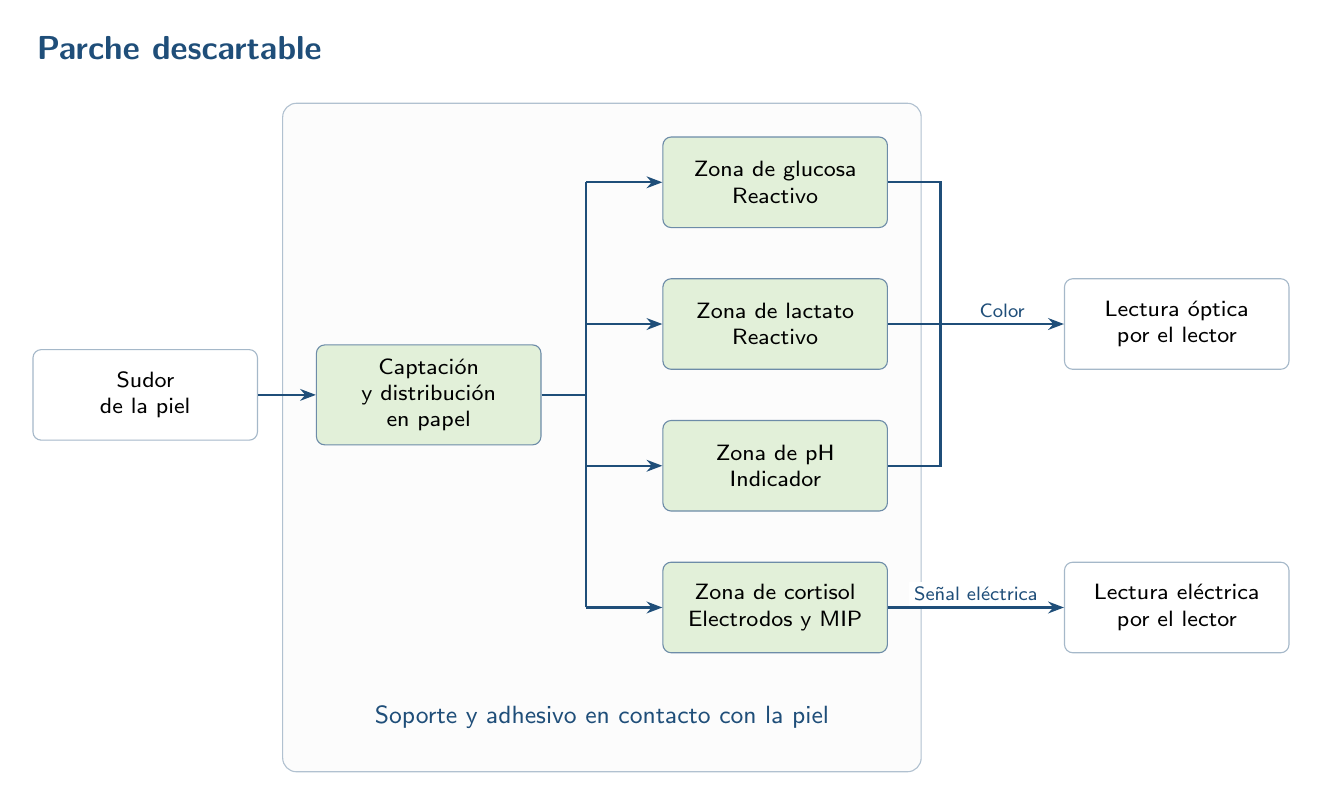
\begin{tikzpicture}
    \node[titulo] at (-1.5,4.4) {Parche descartable};
    \node[externo] (sudor) at (0,0) {Sudor\\de la piel};
    \node[sensor] (cap) at (3.6,0) {Captación\\y distribución\\en papel};
    \node[sensor] (glu) at (8,2.7) {Zona de glucosa\\Reactivo};
    \node[sensor] (lac) at (8,.9) {Zona de lactato\\Reactivo};
    \node[sensor] (ph) at (8,-.9) {Zona de pH\\Indicador};
    \node[sensor] (cor) at (8,-2.7) {Zona de cortisol\\Electrodos y MIP};
    \node[externo] (opt) at (13.1,.9) {Lectura óptica\\por el lector};
    \node[externo] (ele) at (13.1,-2.7) {Lectura eléctrica\\por el lector};
    \draw[flujo] (sudor)--(cap);
    \draw[relacion] (cap.east)--(5.6,0);
    \draw[relacion] (5.6,-2.7)--(5.6,2.7);
    \foreach \n in {glu,lac,ph,cor} {\draw[flujo] (5.6,0|-\n.west)--(\n.west);}
    \draw[relacion] (glu.east)--(10.1,2.7)--(10.1,-.9)--(ph.east);
    \draw[relacion] (lac.east)--(10.1,.9);
    \draw[flujo] (10.1,.9)--node[rotulo,above]{Color}(opt.west);
    \draw[flujo] (cor.east)--node[rotulo,above]{Señal eléctrica}(ele.west);
    \node[font=\sffamily\small,text=tpazul] (base) at (5.8,-4.1) {Soporte y adhesivo en contacto con la piel};
    \begin{scope}[on background layer]
        \node[marco,fit=(cap)(glu)(lac)(ph)(cor)(base)] {};
    \end{scope}
    \end{tikzpicture}}
    \caption{Esquema funcional del parche sensor descartable: captación y distribución del sudor, zonas de sensado y lecturas óptica y electroquímica realizadas por el módulo reutilizable.}
    \label{fig:parche-descartable}
\end{figure}



\begin{figure}[H]
\centering
\resizebox{\linewidth}{!}{%
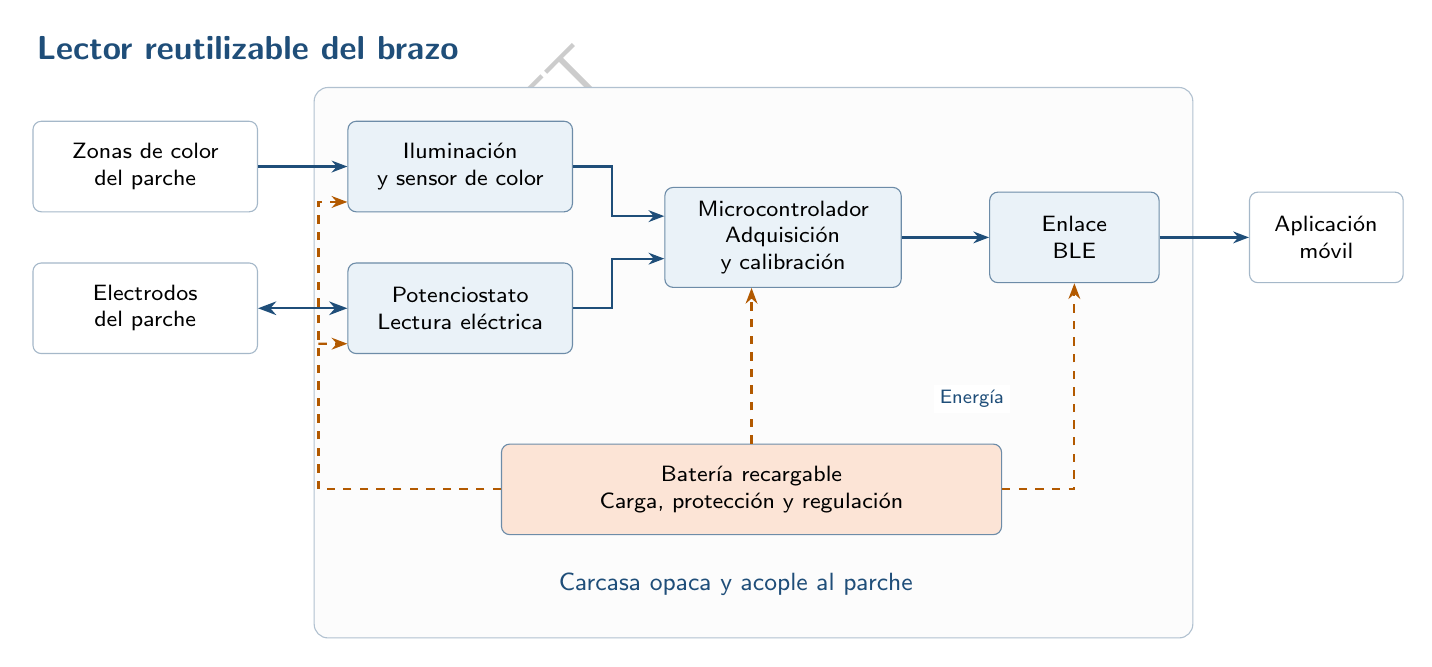
\begin{tikzpicture}
\node[titulo] at (-1.5,2.4) {Lector reutilizable del brazo};
\node[externo] (color) at (0,.9) {Zonas de color\\del parche};
\node[externo] (cort) at (0,-.9) {Electrodos\\del parche};
\node[bloque] (optica) at (4,.9) {Iluminación\\y sensor de color};
\node[bloque] (pot) at (4,-.9) {Potenciostato\\Lectura eléctrica};
\node[bloque,text width=2.65cm] (mc) at (8.1,0) {Microcontrolador\\Adquisición\\y calibración};
\node[bloque,text width=1.8cm] (ble) at (11.8,0) {Enlace\\BLE};
\node[externo,text width=1.6cm] (app) at (15,0) {Aplicación\\móvil};
\node[energia,text width=6cm] (pwr) at (7.7,-3.2) {Batería recargable\\Carga, protección y regulación};
\draw[flujo] (color)--(optica);
\draw[flujo,arrows={Stealth-Stealth}] (cort)--(pot);
\draw[flujo] (optica.east)--++(.5,0)|-([yshift=.27cm]mc.west);
\draw[flujo] (pot.east)--++(.5,0)|-([yshift=-.27cm]mc.west);
\draw[flujo] (mc)--(ble);
\draw[flujo] (ble)--(app);
\draw[potencia] (pwr.north)--(pwr.north|-mc.south);
\draw[potencia] (pwr.west)--(2.2,-3.2)--(2.2,.45)--([yshift=-.45cm]optica.west);
\draw[potencia] (2.2,-1.35)--([yshift=-.45cm]pot.west);
\draw[potencia] (pwr.east)-|(ble.south);
\node[rotulo] at (10.5,-2.05) {Energía};
\node[font=\sffamily\small,text=tpazul] (base) at (7.5,-4.4) {Carcasa opaca y acople al parche};
\begin{scope}[on background layer]
\node[marco,fit=(optica)(pot)(mc)(ble)(pwr)(base)] {};
\end{scope}
\end{tikzpicture}}
\caption{Diagrama de bloques del lector reutilizable del brazo. Las flechas discontinuas indican alimentación eléctrica. Fuente: elaboración propia.}
\label{fig:lector-reutilizable}
\end{figure}


\begin{figure}[H]
\centering
\resizebox{\linewidth}{!}{%
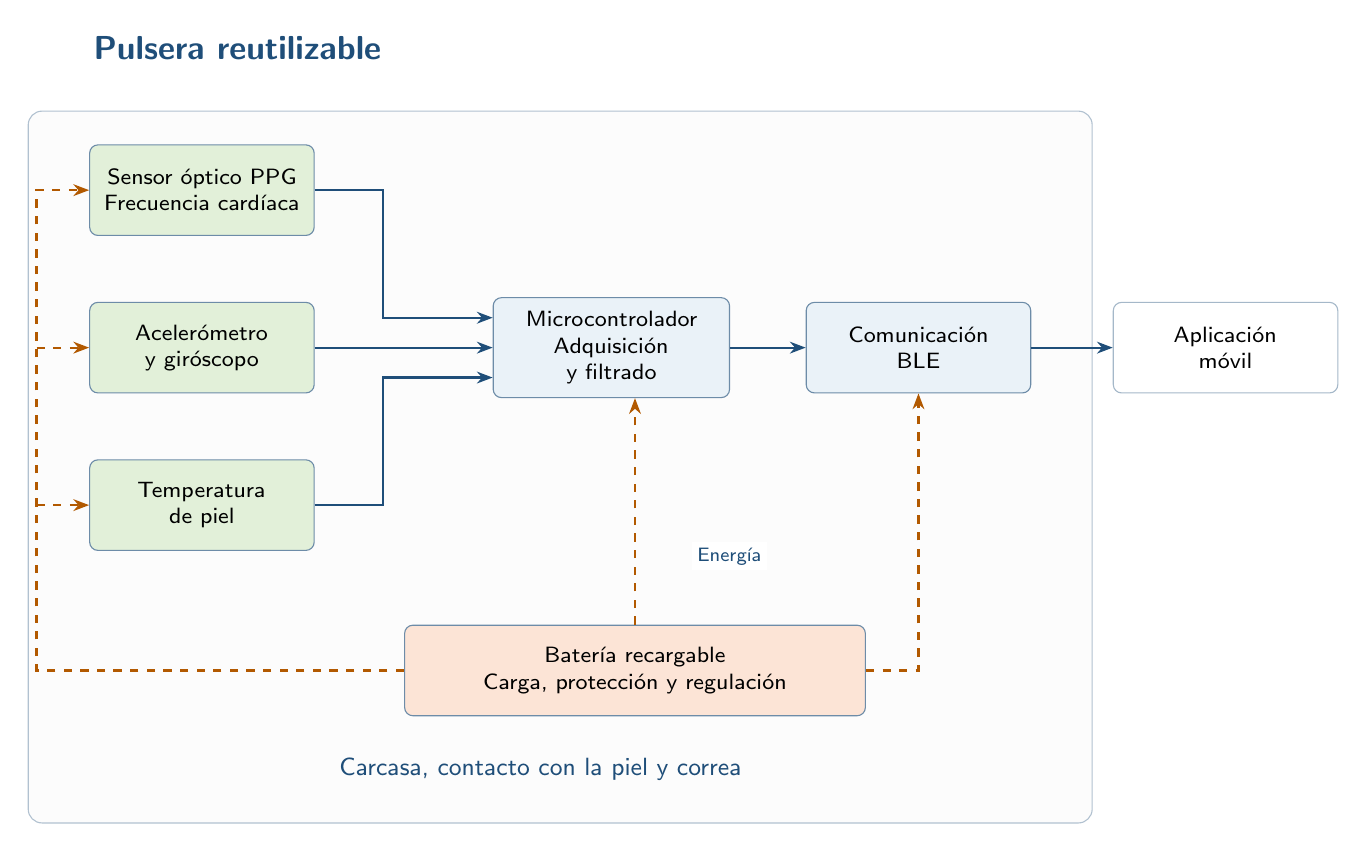
\begin{tikzpicture}
\node[titulo] at (-1.5,4.3) {Pulsera reutilizable};
\node[sensor] (ppg) at (0,2.5) {Sensor óptico PPG\\Frecuencia cardíaca};
\node[sensor] (imu) at (0,.5) {Acelerómetro\\y giróscopo};
\node[sensor] (tmp) at (0,-1.5) {Temperatura\\de piel};
\node[bloque,text width=2.65cm] (mc) at (5.2,.5) {Microcontrolador\\Adquisición\\y filtrado};
\node[bloque] (ble) at (9.1,.5) {Comunicación\\BLE};
\node[externo] (app) at (13,.5) {Aplicación\\móvil};
\node[energia,text width=5.5cm] (pwr) at (5.5,-3.6) {Batería recargable\\Carga, protección y regulación};
\draw[flujo] (ppg.east)--(2.3,2.5)|-([yshift=.38cm]mc.west);
\draw[flujo] (imu)--(mc);
\draw[flujo] (tmp.east)--(2.3,-1.5)|-([yshift=-.38cm]mc.west);
\draw[flujo] (mc)--(ble);
\draw[flujo] (ble)--(app);
\draw[potencia] (pwr.north)--(pwr.north|-mc.south);
\draw[potencia] (pwr.east)-|(ble.south);
\draw[potencia] (pwr.west)--(-2.1,-3.6)--(-2.1,2.5)--(ppg.west);
\draw[potencia] (-2.1,.5)--(imu.west);
\draw[potencia] (-2.1,-1.5)--(tmp.west);
\node[rotulo] at (6.7,-2.15) {Energía};
\node[font=\sffamily\small,text=tpazul] (base) at (4.3,-4.85) {Carcasa, contacto con la piel y correa};
\begin{scope}[on background layer]
\node[marco,fit=(ppg)(imu)(tmp)(mc)(ble)(pwr)(base),inner xsep=22pt] {};
\end{scope}
\end{tikzpicture}}
\caption{Diagrama de bloques de la pulsera reutilizable. Las flechas discontinuas indican alimentación eléctrica. Fuente: elaboración propia.}
\label{fig:pulsera-reutilizable}
\end{figure}



\begin{figure}[H]
\centering
\resizebox{\linewidth}{!}{%
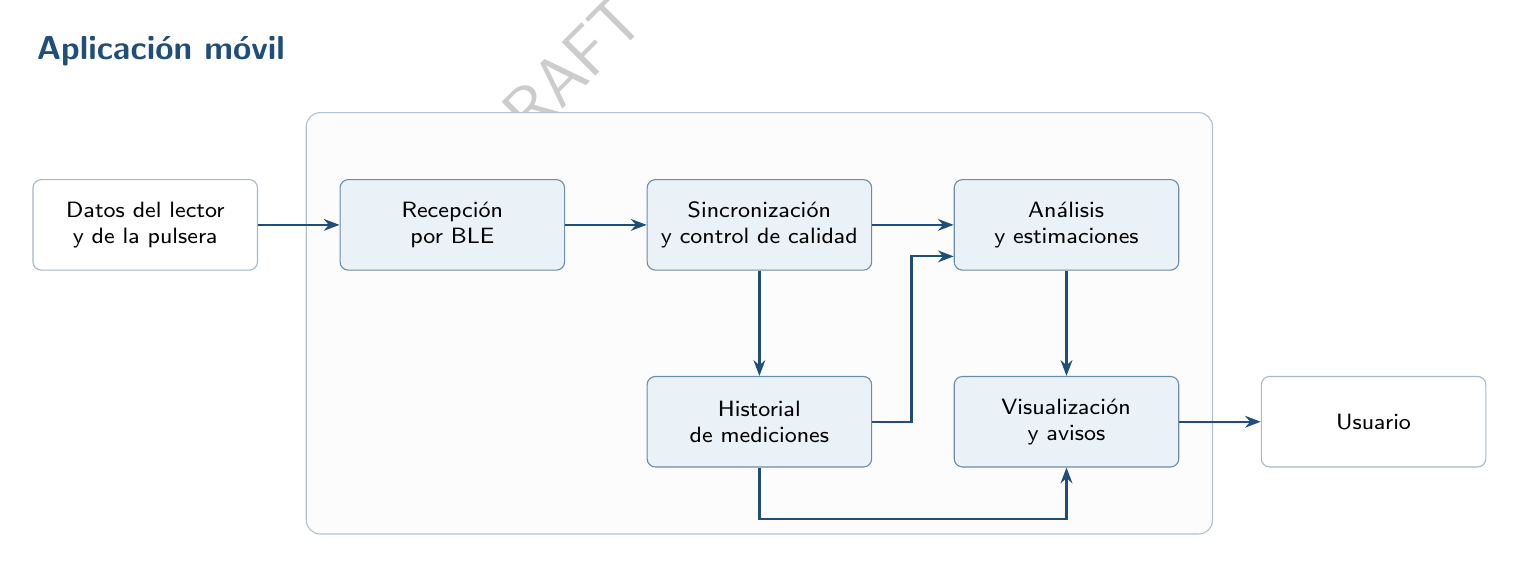
\begin{tikzpicture}
\node[titulo] at (-1.5,2.2) {Aplicación móvil};
\node[externo] (in) at (0,0) {Datos del lector\\y de la pulsera};
\node[bloque] (rx) at (3.9,0) {Recepción\\por BLE};
\node[bloque] (prep) at (7.8,0) {Sincronización\\y control de calidad};
\node[bloque] (model) at (11.7,0) {Análisis\\y estimaciones};
\node[bloque] (hist) at (7.8,-2.5) {Historial\\de mediciones};
\node[bloque] (ui) at (11.7,-2.5) {Visualización\\y avisos};
\node[externo] (usr) at (15.6,-2.5) {Usuario};
\draw[flujo] (in)--(rx);
\draw[flujo] (rx)--(prep);
\draw[flujo] (prep)--(model);
\draw[flujo] (prep)--(hist);
\draw[flujo] (hist.east)--++(.5,0)|-([yshift=-.4cm]model.west);
\draw[flujo] (model)--(ui);
\draw[flujo] (hist.south)--++(0,-.65)-|(ui.south);
\draw[flujo] (ui)--(usr);
\begin{scope}[on background layer]
\node[marco,fit=(rx)(prep)(model)(hist)(ui),inner ysep=24pt] {};
\end{scope}
\end{tikzpicture}}
\caption{Diagrama funcional de la aplicación móvil. El análisis podrá ejecutarse en el teléfono o mediante un servicio remoto, según la alternativa seleccionada. Fuente: elaboración propia.}
\label{fig:aplicacion-movil}
\end{figure}

\begin{figure}[H]
\centering
\resizebox{\linewidth}{!}{%
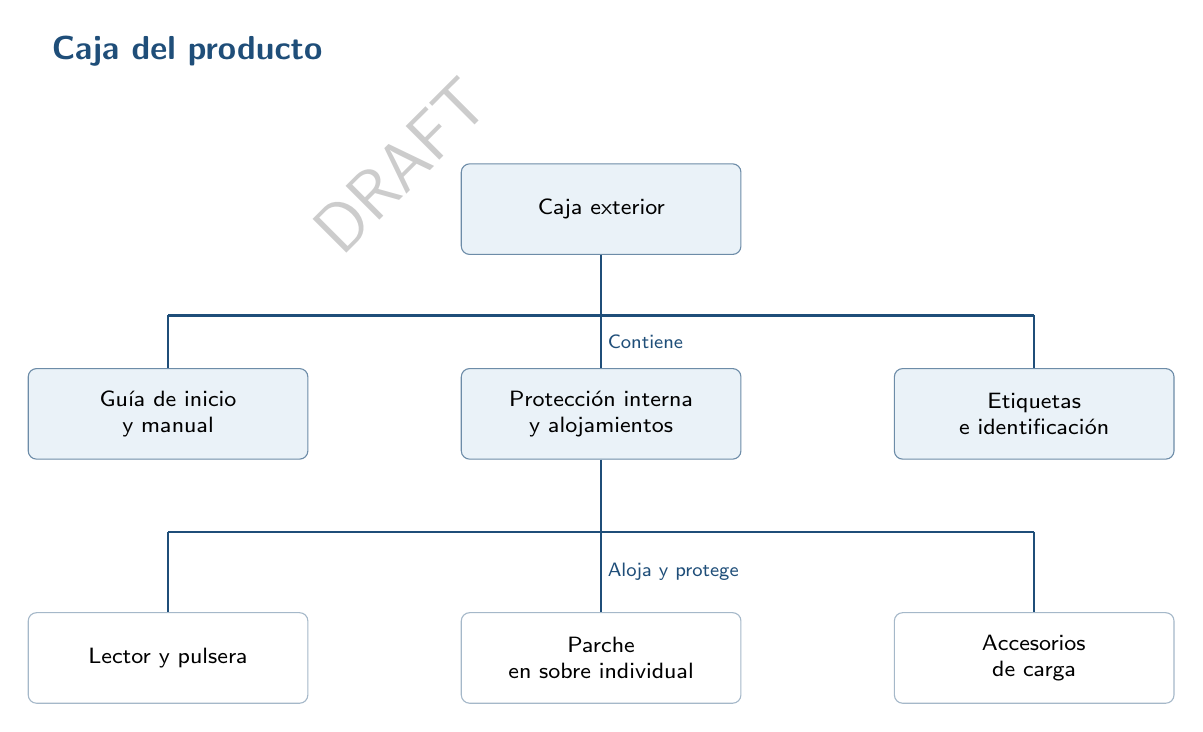
\begin{tikzpicture}
\node[titulo] at (-1.6,2.3) {Caja del producto};
\node[bloque,text width=3.2cm] (caja) at (5.5,.3) {Caja exterior};
\node[bloque,text width=3.2cm] (guia) at (0,-2.3) {Guía de inicio\\y manual};
\node[bloque,text width=3.2cm] (proteccion) at (5.5,-2.3) {Protección interna\\y alojamientos};
\node[bloque,text width=3.2cm] (etiqueta) at (11,-2.3) {Etiquetas\\e identificación};
\node[externo,text width=3.2cm] (equipos) at (0,-5.4) {Lector y pulsera};
\node[externo,text width=3.2cm] (parche) at (5.5,-5.4) {Parche\\en sobre individual};
\node[externo,text width=3.2cm] (accesorios) at (11,-5.4) {Accesorios\\de carga};
\draw[relacion] (caja.south)--(5.5,-1.05);
\draw[relacion] (0,-1.05)--(11,-1.05);
\draw[relacion] (0,-1.05)--(guia.north);
\draw[relacion] (5.5,-1.05)--node[rotulo,right]{Contiene}(proteccion.north);
\draw[relacion] (11,-1.05)--(etiqueta.north);
\draw[relacion] (proteccion.south)--(5.5,-3.8);
\draw[relacion] (0,-3.8)--(11,-3.8);
\draw[relacion] (0,-3.8)--(equipos.north);
\draw[relacion] (5.5,-3.8)--node[rotulo,right]{Aloja y protege}(parche.north);
\draw[relacion] (11,-3.8)--(accesorios.north);
\end{tikzpicture}}
\caption{Organización preliminar del paquete del sensor. Las líneas indican relaciones de contenido y alojamiento. Fuente: elaboración propia.}
\label{fig:caja-producto}
\end{figure}




Las listas de componentes y sus costos se presentan en las Tablas~\ref{tab:costo-parche}, \ref{tab:costo-lector}, \ref{tab:costo-pulsera} y \ref{tab:costo-caja}; la Tabla~\ref{tab:costo-app} detalla el trabajo de implementación de la aplicación.

\FloatBarrier
\paragraph{Análisis AMFE (preliminar)}
\label{sec:amfe-preliminar}
{\consigna
Aquí debe incorporarse el Análisis AMFE preliminar e ir enriqueciéndolo a lo largo del diseño y desarrollo del proyecto.
}


{\footnotesize
\renewcommand{\arraystretch}{1.2}
\begin{longtable}{|>{\raggedright\arraybackslash}p{\dimexpr0.18\textwidth-2\tabcolsep-1.2\arrayrulewidth\relax}|>{\raggedright\arraybackslash}p{\dimexpr0.22\textwidth-2\tabcolsep-1.2\arrayrulewidth\relax}|>{\raggedright\arraybackslash}p{\dimexpr0.18\textwidth-2\tabcolsep-1.2\arrayrulewidth\relax}|>{\raggedright\arraybackslash}p{\dimexpr0.13\textwidth-2\tabcolsep-1.2\arrayrulewidth\relax}|>{\raggedright\arraybackslash}p{\dimexpr0.29\textwidth-2\tabcolsep-1.2\arrayrulewidth\relax}|}
\hline
\textbf{Componente / función} & \textbf{Modo de falla} & \textbf{Efecto} & \textbf{Severidad} & \textbf{Mitigación propuesta} \\
\hline
\endfirsthead
\hline
\textbf{Componente / función} & \textbf{Modo de falla} & \textbf{Efecto} & \textbf{Severidad} & \textbf{Mitigación propuesta} \\
\hline
\endhead
Zonas colorimétricas (glucosa, lactato, pH) & Interferencia por condiciones de luz ambiente al leer el color & Medición imprecisa & Media & Lector con carcasa que aísla luz ambiente, o calibración por referencia de color interna \\
\hline
Zonas colorimétricas & Degradación del reactivo cromogénico por humedad o tiempo de almacenamiento & Lectura nula o errónea & Media & Empaque sellado, indicación de vida útil, control de lote en fabricación \\
\hline
Secuenciado de reacciones (plegado de papel) & Plegado incorrecto por parte del usuario al colocar el parche sensor descartable & Mezcla de zonas, lectura cruzada & Media & Diseño de plegado guiado mecánicamente (una sola forma posible de doblar) \\
\hline
Zona cortisol (MIP electroquímico) & Baja especificidad, interferencia de otras moléculas del sudor & Asociación incorrecta con estrés & Media & Evaluar especificidad y contrastar con señales de contexto; no presentar el resultado como diagnóstico ni como causalidad clínica \\
\hline
Comunicación BLE & Pérdida de conexión entre dispositivo y hub & Interrupción de datos o aviso no emitido & Media & Sincronización cada 5 min y alcance objetivo de hasta 10 m (incluido teléfono en bolsillo), a validar; buffer local de 24 h (45 KiB/día por dispositivo) y envío en bloque al reconectar; advertir intervalos faltantes si se excede el buffer \\
\hline
Batería (módulo electrónico reutilizable o pulsera) & Descarga antes de lo esperado & Vacío de datos, pérdida de contexto & Media & Diseño de bajo consumo e indicador de batería baja; verificar autonomía objetivo de 7 días en el perfil nominal de uso \\
\hline
Modelo de factores asociados (IA) & Asociación incorrecta entre una variación y un factor de contexto & Información o aviso inadecuado al usuario & Alta & Presentar factores como probablemente asociados, informar incertidumbre y evitar inferencias causales o recomendaciones automáticas de tratamiento \\
\hline
\end{longtable}
}

\subsubsection{Inventario de los diferentes aspectos a cubrir}
{\consigna
En este apartado debe enumerarse y describirse todos los aspectos involucrados en el proyecto que son necesarios para cumplir el objetivo.\\
Dependiendo del objetivo, será la cantidad de aspectos a tener en cuenta.\\
Se mencionan algunos ejemplos que podrían aplicar:

\begin{itemize}
\setlength{\itemsep}{3 pt}
    \item Línea de Producción / fabricación
    \item QA
    \item Soporte
    \item Repuestos, Entrenamiento
    \item Servicios Especializados
\end{itemize}
}


\begin{itemize}
    \item \textbf{Línea de producción/fabricación:} fabricación de parches sensores descartables de papel plegado (microfluídica de papel), incluidas sus zonas con reactivos y su soporte adhesivo, y ensamblado del módulo electrónico reutilizable de lectura óptica/electroquímica y comunicación y de la pulsera reutilizable.
    \item \textbf{QA:} control de calidad por lote de reactivos cromogénicos, calibración de color de cada lector, calibración de cada unidad de pulsera.
    \item \textbf{Soporte:} atención a usuarios ante fallas de sincronización, dudas sobre plegado y recambio del parche sensor descartable, acoplamiento del módulo electrónico reutilizable o interpretación de la información y los avisos; mantenimiento del módulo electrónico y de la pulsera reutilizables y actualización de firmware remota.
    \item \textbf{Repuestos:} provisión y recambio del parche sensor descartable completo (papel, zonas con reactivos y soporte adhesivo), con recambio objetivo cada 7 días.
    \item \textbf{Entrenamiento:} capacitación a usuarios y profesionales para efectuar el recambio del parche sensor y el acoplamiento del módulo electrónico, e interpretar las mediciones, estimaciones, incertidumbres y avisos dentro del uso previsto.
    \item \textbf{Servicios especializados:} laboratorio de química/bioquímica para seleccionar reactivos cromogénicos existentes, adaptar su formulación e inmovilización en el soporte de papel y validar su desempeño en sudor; para la zona de cortisol, preparación e integración del MIP a partir de protocolos publicados, con evaluación de selectividad y estabilidad. No se plantea desarrollar nuevas químicas de detección desde cero, sino adaptar soluciones existentes al dispositivo propuesto.
\end{itemize}

\subsection{Evaluación de factibilidad de negocio}
{\consigna
Esta sección aborda la evaluación de Negocio, analizando los aspectos relacionados con la receptividad o posibilidades de adopción del resultado del proyecto por parte de los destinatarios del mismo y las posibilidades de realización desde lo organizacional, legal, económico y demás cuestiones no tecnológicas que deban considerarse.
}




\subsubsection{Análisis FODA}
{\consigna
Esta sección incorpora un análisis FODA del proyecto (del resultado del proyecto).\\
Esta sección, como todas, es dinámica y se enriquece a lo largo del desarrollo del proyecto.
}

El análisis considera el alcance conceptual actual del proyecto. Las fortalezas se plantean como ventajas internas esperadas del producto. Las oportunidades corresponden a condiciones externas que podrían favorecer su desarrollo o adopción.

\noindent\textbf{Fortalezas}
\begin{itemize}
    \item Más contexto e información relevante para interpretar las variaciones de glucosa: el producto ofrece información sobre factores probablemente asociados, como alimentación, estrés o actividad física, para que el usuario no tenga que interpretar únicamente un número/historial por su cuenta. Esta información complementa el seguimiento con CGM, sin constituir un diagnóstico de la causa.
    \item Menor esfuerzo de registro frente a la transcripción manual de mediciones: la recepción automática de datos del módulo electrónico reutilizable y la pulsera y su organización en un historial común evitan que el usuario copie y reúna esas mediciones por su cuenta para consultar su evolución.
    \item Seguimiento de varios biomarcadores en sudor sin punciones ni extracción de sangre para obtener esas mediciones, como alternativa no invasiva para reunir información metabólica adicional. Esta ventaja no implica sustituir los controles sanguíneos ni el CGM.
    \item Reutilización de la electrónica. El módulo lector y la pulsera se conservan al reemplazar el parche sensor descartable, por lo que el costo de reposición corresponde al consumible y su empaque. 
\end{itemize}

\noindent\textbf{Oportunidades}
\begin{itemize}
    \item Posibilidad de atender a personas con diabetes tipo 2 o prediabetes que busquen comprender mejor la relación entre sus hábitos cotidianos y las variaciones de glucosa, mediante una propuesta de seguimiento complementario y personalizado.
    \item Posibilidad de establecer alianzas con clínicas y profesionales de salud interesados en evaluar herramientas de seguimiento entre consultas, validar la utilidad de la información contextual y definir cómo presentar los avisos.
    \item Interés en el uso de biomarcadores para el monitoreo de enfermedades crónicas.
\end{itemize}

\noindent\textbf{Debilidades}
\begin{itemize}
    \item Experiencia y recursos especializados limitados: el equipo no cuenta actualmente con experiencia práctica demostrada, antecedentes propios ni infraestructura especializada para desarrollar y validar sensores bioquímicos, dispositivos médicos y modelos de inteligencia artificial aplicados a información clínica. También carece de experiencia directa en validación clínica y procesos regulatorios, por lo que dependerá de laboratorios, profesionales de salud e instituciones externas para cubrir estas capacidades.
    \item Experiencia limitada del equipo en el desarrollo integral de dispositivos médicos: como estudiantes de Ingeniería Electrónica, los integrantes cuentan con formación teórica en electrónica, pero aún deben adquirir experiencia práctica en su aplicación al diseño de dispositivos médicos. También será necesario ampliar conocimientos en biosensores, modelos de IA, validación clínica, regulación e industrialización, mediante aprendizaje específico, asesoramiento especializado y alianzas con profesionales de esas áreas.
    \item Desempeño aún no demostrado: el proyecto no cuenta con un prototipo integrado ni validación propia que permita comprobar la calidad de las mediciones y de las predicciones propuestas.
    \item La colocación del parche sensor descartable, el acoplamiento del módulo electrónico reutilizable y el uso conjunto con la pulsera pueden resultar complejos para el usuario, lo que podría dificultar la utilización adecuada del sistema.
\end{itemize}

\noindent\textbf{Amenazas}
\begin{itemize}
    \item Disponibilidad o acceso insuficiente a datos adecuados para la IA: la falta de registros sincronizados de biomarcadores, señales fisiológicas y eventos de referencia podría limitar el entrenamiento y la evaluación de los modelos, comprometiendo la confiabilidad de la información ofrecida por el producto. Si se determina que los modelos requieren datos de un CGM, las restricciones de acceso a esos registros podrían agravar esta limitación.
    \item Riesgo de dificultades en la integración y calibración: la coordinación de lecturas colorimétricas, electroquímicas y fisiológicas podría no alcanzar la consistencia requerida, comprometiendo el desempeño del sistema y aumentando los plazos y costos de desarrollo.
    \item Fabricantes de CGM u otros desarrolladores podrían incorporar funciones de interpretación contextual o asociación de eventos antes de que el proyecto alcance una versión comercial, reduciendo su diferenciación.
    \item Las exigencias de evidencia, seguridad y autorización que resulten aplicables al uso previsto podrían extender los plazos y aumentar los costos del desarrollo. La clasificación regulatoria deberá confirmarse y no se considera resuelta por utilizar una tecnología de sensado determinada.
    \item Usuarios y posibles financiadores de la compra, como obras sociales o aseguradoras, podrían no considerar suficiente el beneficio adicional frente al costo del sistema y al recambio de parches sensores descartables, con recambio objetivo cada 7 días, sujeto a validar su estabilidad, adhesión y desempeño, limitando su adopción incluso si la solución resulta técnicamente viable.
    \item La falta de acceso a financiamiento externo o a acuerdos con instituciones para realizar ensayos y obtener datos podría demorar el paso del diseño conceptual a un prototipo validado.
\end{itemize}




\subsubsection{Análisis de Riesgos}
{\consigna
En esta sección se deben identificar los riesgos del proyecto, es decir, todos los factores que puedan atentar contra el éxito del mismo.\\
Hemos dividido el análisis en dos partes: Matriz de Riesgos y Análisis AMFE.
}

Este análisis cubre las debilidades y amenazas identificadas en el FODA que podrían afectar la preparación y la continuidad del proyecto. Los modos de falla del producto se tratan en el AMFE de la sección~\ref{sec:amfe-preliminar}.

\noindent\textbf{a) Identificación de los riesgos}
\begin{itemize}
    \item R1 $\rightarrow$ Evidencia insuficiente o dificultades de integración y calibración que impidan sustentar la factibilidad técnica del sensado.
    \item R2 $\rightarrow$ Falta de acceso a datos sincronizados y adecuados para especificar y evaluar los modelos de IA, incluidos datos de CGM si finalmente fueran necesarios.
    \item R3 $\rightarrow$ Falta de experiencia especializada, asesoramiento, infraestructura o financiamiento externo para desarrollar el análisis y dar continuidad a la validación posterior.
    \item R4 $\rightarrow$ Subestimación del esfuerzo y cambios tardíos de alcance que retrasen o dejen incompletos los entregables.
    \item R5 $\rightarrow$ Inconsistencias entre el diseño técnico, los supuestos y las conclusiones de factibilidad y negocio.
    \item R6 $\rightarrow$ Entrada o avance de competidores que reduzca la diferenciación de la propuesta antes de una eventual etapa de desarrollo posterior.
    \item R7 $\rightarrow$ Baja aceptación por la complejidad de uso, el uso combinado de parche y pulsera o el costo y recambio periódico del parche sensor.
    \item R8 $\rightarrow$ Incertidumbre sobre los requisitos de evidencia, seguridad y autorización aplicables al uso previsto, que afecte la evaluación regulatoria y la planificación de etapas posteriores.
\end{itemize}

\noindent\textbf{b) Estimación de las consecuencias de los riesgos}

Se propone una escala ordinal de 1 a 10. La severidad ($S$) estima el impacto sobre el proyecto o sus entregables; la ocurrencia ($O$) estima la posibilidad de que el riesgo se materialice. $O$ no representa un porcentaje. Las puntuaciones son estimaciones preliminares para revisar con el equipo, no frecuencias observadas ni resultados validados.

\noindent R1 $\rightarrow$ Evidencia e integración técnica.
\begin{itemize}
    \item Severidad ($S$): 9, porque podría impedir fundamentar la arquitectura o concluir sobre la factibilidad de las mediciones propuestas.
    \item Ocurrencia ($O$): 6, porque los rangos, interferencias, estabilidad de los reactivos, calibración e integración de las lecturas todavía requieren análisis y contraste.
\end{itemize}

\noindent R2 $\rightarrow$ Disponibilidad de datos para IA.
\begin{itemize}
    \item Severidad ($S$): 8, porque dejaría incompletas la especificación de los modelos y la justificación de su evaluación.
    \item Ocurrencia ($O$): 6, porque todavía no se identificó una fuente confirmada de registros sincronizados con las variables y referencias necesarias.
\end{itemize}

\noindent R3 $\rightarrow$ Experiencia y recursos especializados.
\begin{itemize}
    \item Severidad ($S$): 8, porque la falta de especialistas o recursos podría limitar el análisis de biosensores, IA, validación y regulación, así como postergar una eventual etapa de validación.
    \item Ocurrencia ($O$): 6, porque el equipo aún debe adquirir experiencia práctica y depende de asesoramiento, laboratorios y posibles acuerdos o fondos externos.
\end{itemize}

\noindent R4 $\rightarrow$ Esfuerzo, plazos y alcance.
\begin{itemize}
    \item Severidad ($S$): 7, porque podría producir entregables incompletos o reducir el tiempo de integración y revisión.
    \item Ocurrencia ($O$): 5, porque el trabajo combina disciplinas con dependencias entre sí y el alcance puede cambiar a medida que se revisa la evidencia.
\end{itemize}

\noindent R5 $\rightarrow$ Coherencia entre secciones.
\begin{itemize}
    \item Severidad ($S$): 6, porque las contradicciones entre requisitos, diseño, AMFE, mercado y factibilidad debilitarían la trazabilidad y las conclusiones.
    \item Ocurrencia ($O$): 5, porque las iteraciones del diseño y las distintas secciones pueden dejar supuestos o especificaciones desactualizados.
\end{itemize}

\noindent R6 $\rightarrow$ Cambios en el entorno competitivo.
\begin{itemize}
    \item Severidad ($S$): 6, porque una oferta similar podría reducir la diferenciación prevista para una eventual continuidad comercial.
    \item Ocurrencia ($O$): 4, como estimación preliminar ante un entorno competitivo cambiante; no implica que se haya confirmado la entrada de un competidor.
\end{itemize}

\noindent R7 $\rightarrow$ Aceptación y uso del sistema.
\begin{itemize}
    \item Severidad ($S$): 7, porque una experiencia difícil o un costo recurrente que el usuario no acepte limitaría la adopción, aunque el diseño técnico resultara viable.
    \item Ocurrencia ($O$): 5, porque el uso conjunto de los dispositivos, la colocación y el acoplamiento del parche y su recambio todavía no se evaluaron con usuarios.
\end{itemize}

\noindent R8 $\rightarrow$ Incertidumbre regulatoria.
\begin{itemize}
    \item Severidad ($S$): 8, porque requisitos no identificados podrían cambiar el uso previsto, la evidencia necesaria, los plazos y los costos de una etapa posterior.
    \item Ocurrencia ($O$): 5, porque la clasificación y los requisitos aplicables dependen del uso previsto y todavía deben confirmarse mediante análisis especializado.
\end{itemize}

    \paragraph{Matriz de Riesgos y Acciones de Mitigación}
    {\consigna
    Aquí debe incorporarse la Matriz de Riesgos y las Acciones Mitigadoras a tomar.\\
    Esta parte se irá completando a lo largo del diseño preliminar y las demás secciones.\\
    El alumno debe investigar diferentes modelos de matrices de riesgos y elegir la que mejor aplique a su proyecto.
    }

\noindent\textbf{c) Tabla de gestión de riesgos}

Se utiliza el índice de prioridad definido para este análisis como $\mathrm{RPN} = S \times O$. Se propone un umbral máximo aceptable de 25; tanto el umbral como las puntuaciones son criterios preliminares del equipo.

{\small
\renewcommand{\arraystretch}{1.2}
\noindent\begin{tabularx}{\textwidth}{|*{4}{>{\centering\arraybackslash}X|}}
\hline
\textbf{Riesgo} & $S$ & $O$ & \textbf{RPN} \\
\hline
R1 & 9 & 6 & 54 \\
\hline
R2 & 8 & 6 & 48 \\
\hline
R3 & 8 & 6 & 48 \\
\hline
R4 & 7 & 5 & 35 \\
\hline
R5 & 6 & 5 & 30 \\
\hline
R6 & 6 & 4 & 24 \\
\hline
R7 & 7 & 5 & 35 \\
\hline
R8 & 8 & 5 & 40 \\
\hline
\end{tabularx}
\par}

Se definen acciones para R1--R5, R7 y R8 por superar el umbral propuesto. R6 se acepta provisionalmente con seguimiento, dado que su RPN está por debajo del umbral; se revisará si aparecen indicios concretos de cambios competitivos relevantes.

\noindent\textbf{d) Plan de mitigación de los riesgos que superan el umbral}

Las puntuaciones residuales expresan objetivos preliminares después de aplicar las acciones, no reducciones comprobadas. Los riesgos cuyo RPN residual siga por encima del umbral deberán mantenerse abiertos y revisarse; una matriz no elimina la incertidumbre técnica, de mercado ni regulatoria.

\noindent R1 $\rightarrow$ Mitigación de la incertidumbre técnica.
\begin{itemize}
    \item Acción: revisar la evidencia de cada zona de sensado y registrar principio de medición, rango, condiciones de ensayo, interferencias y limitaciones. Construir un prototipo integrado de alcance acotado y realizar pruebas preliminares de adquisición, integración y calibración; registrar resultados y desvíos, priorizar ajustes y repetir las pruebas pertinentes. Distinguir las mediciones en sudor de cualquier estimación de glucosa sanguínea. Las pruebas del prototipo no equivalen a validación clínica ni demuestran por sí solas la precisión de los modelos de IA; si persisten brechas, documentarlas como limitaciones en vez de presentar la factibilidad como demostrada.
    \item Severidad residual ($S^{*}$): 9. Se mantiene el impacto si la evidencia no sustenta la solución.
    \item Ocurrencia residual objetivo ($O^{*}$): 4, condicionado a la revisión documentada.
    \item $\mathrm{RPN}^{*} = 36$; permanece sobre el umbral y requiere seguimiento.
\end{itemize}

\noindent R2 $\rightarrow$ Mitigación de la incertidumbre sobre datos.
\begin{itemize}
    \item Acción: identificar las fuentes disponibles, variables, sincronización, referencias y condiciones de acceso. Aclarar si los modelos requerirían datos de un CGM y cómo se integrarían. Especificar por separado la evaluación de ambos horizontes temporales y de los factores asociados; documentar los datos que faltarían para una validación posterior sin atribuir validación a datos parciales.
    \item Severidad residual ($S^{*}$): 8. Se mantiene el impacto si no se obtienen datos adecuados.
    \item Ocurrencia residual objetivo ($O^{*}$): 4, sujeto a confirmar fuentes y condiciones de acceso.
    \item $\mathrm{RPN}^{*} = 32$; permanece sobre el umbral y requiere seguimiento.
\end{itemize}

\noindent R3 $\rightarrow$ Mitigación de la dependencia de recursos externos.
\begin{itemize}
    \item Acción: identificar qué conocimientos y recursos requiere cada entregable; solicitar revisión a docentes y profesionales, y relevar posibles laboratorios, universidades y fuentes de financiamiento para una futura validación. Asignar responsables y fechas internas; si un recurso no se consigue, explicitar el límite y no presentar como realizado el trabajo que dependa de él.
    \item Severidad residual ($S^{*}$): 8. Se mantiene el impacto de no disponer de recursos especializados.
    \item Ocurrencia residual objetivo ($O^{*}$): 4, condicionada a identificar alternativas y confirmar su disponibilidad.
    \item $\mathrm{RPN}^{*} = 32$; permanece sobre el umbral y requiere seguimiento.
\end{itemize}

\noindent R4 $\rightarrow$ Mitigación de plazos y cambios de alcance.
\begin{itemize}
    \item Acción: dividir el trabajo por entregables, asignar responsables y fechas internas, revisar el avance periódicamente y registrar cambios de alcance con su impacto en plazos y documentos relacionados.
    \item Severidad residual ($S^{*}$): 7. Se mantiene el impacto de una demora.
    \item Ocurrencia residual objetivo ($O^{*}$): 3, condicionada al seguimiento de avance y cambios.
    \item $\mathrm{RPN}^{*} = 21$.
\end{itemize}

\noindent R5 $\rightarrow$ Mitigación de inconsistencias.
\begin{itemize}
    \item Acción: mantener trazabilidad entre objetivo, requerimientos, componentes y entregables; realizar una revisión cruzada del diseño, AMFE, mercado y factibilidad antes de cerrar cada versión. Separar supuestos, evidencia disponible y aspectos pendientes.
    \item Severidad residual ($S^{*}$): 6. Se mantiene el impacto de una contradicción relevante.
    \item Ocurrencia residual objetivo ($O^{*}$): 2, condicionada a la revisión cruzada.
    \item $\mathrm{RPN}^{*} = 12$.
\end{itemize}

\noindent R7 $\rightarrow$ Mitigación de la incertidumbre de uso y aceptación.
\begin{itemize}
    \item Acción: considerar una revisión de usabilidad con usuarios representativos en una etapa posterior; identificar tareas de colocación, acoplamiento, sincronización y recambio. Estimar por separado el costo del módulo reutilizable y el costo recurrente del parche, y presentar su aceptación como una hipótesis pendiente hasta contar con evidencia.
    \item Severidad residual ($S^{*}$): 7. Se mantiene el impacto si la experiencia o el costo no resultan aceptables.
    \item Ocurrencia residual objetivo ($O^{*}$): 4, únicamente después de definir y evaluar las tareas y supuestos de costo.
    \item $\mathrm{RPN}^{*} = 28$; permanece sobre el umbral y requiere seguimiento.
\end{itemize}

\noindent R8 $\rightarrow$ Mitigación de la incertidumbre regulatoria.
\begin{itemize}
    \item Acción: describir el uso previsto y las funciones del sistema, identificar las preguntas regulatorias pendientes y solicitar orientación especializada antes de fijar supuestos sobre clasificación, evidencia, plazos o costos. No asumir una categoría regulatoria sin confirmación.
    \item Severidad residual ($S^{*}$): 8. Se mantiene el impacto de un cambio en los requisitos aplicables.
    \item Ocurrencia residual objetivo ($O^{*}$): 4, condicionado a la consulta y a la revisión del uso previsto.
    \item $\mathrm{RPN}^{*} = 32$; permanece sobre el umbral y requiere seguimiento.
\end{itemize}

\noindent\textbf{Tabla final}
\par\medskip
{\small
\renewcommand{\arraystretch}{1.2}
\noindent\begin{tabularx}{\textwidth}{|*{7}{>{\centering\arraybackslash}X|}}
\hline
\textbf{Riesgo} & $S$ & $O$ & \textbf{RPN} & $S^{*}$ & $O^{*}$ & $\mathrm{RPN}^{*}$ \\
\hline
R1 & 9 & 6 & 54 & 9 & 4 & 36 \\
\hline
R2 & 8 & 6 & 48 & 8 & 4 & 32 \\
\hline
R3 & 8 & 6 & 48 & 8 & 4 & 32 \\
\hline
R4 & 7 & 5 & 35 & 7 & 3 & 21 \\
\hline
R5 & 6 & 5 & 30 & 6 & 2 & 12 \\
\hline
R6 & 6 & 4 & 24 & 6 & 4 & 24 \\
\hline
R7 & 7 & 5 & 35 & 7 & 4 & 28 \\
\hline
R8 & 8 & 5 & 40 & 8 & 4 & 32 \\
\hline
\end{tabularx}
\par}

R1, R2, R3, R7 y R8 mantienen un RPN residual por encima del umbral y no se consideran mitigados: deben permanecer abiertos para la siguiente revisión. Para R6 se conservan las puntuaciones iniciales por tratarse de un riesgo aceptado con seguimiento.




\subsection{Análisis de mercado y financiero}
{\consigna
En esta subsección se aborda el mercado destinatario del proyecto, la receptividad a la adopción y los aspectos financieros o de soporte relacionados con la realización y éxito del proyecto.
}

\subsubsection{Análisis de mercado y público objetivo}
{\consigna
En este apartado debe describirse de forma cualitativa quiénes son los usuarios finales del proyecto y quiénes son los adquirentes del proyecto, teniendo en cuenta que pueden diferir.\\
También debe describirse la forma en que ese público satisface actualmente las prestaciones que dará el proyecto y cómo lo hace, cuál es el esfuerzo o costo que asume para ello.\\
También debe dimensionarse de alguna forma el mercado potencial.\\
Luego de leer esta sección, el lector deberá tener un entendimiento holístico del usuario final y adquirente: sus necesidades, expectativas, exigencias y motivaciones relacionadas con el proyecto.
}

Para dimensionar el público potencial en Argentina se toma como referencia la población con diabetes, en lugar de extrapolar directamente la facturación mundial del mercado de monitoreo continuo de glucosa. La Federación Internacional de Diabetes estima que en 2024 había aproximadamente 4,3 millones de personas de entre 20 y 79 años con diabetes en Argentina.\footnote{Federación Internacional de Diabetes, \textit{IDF Diabetes Atlas}, 11.\textsuperscript{a} edición, 2025, capítulo 4: estimaciones para América del Sur y Central correspondientes a 2024.} Como referencia general, la diabetes tipo 2 representa entre el 90\% y el 95\% de los casos de \textit{diabetes mellitus}.\footnote{F. J. Tébar Massó y F. Escobar Jiménez, \textit{La Diabetes en la Práctica Clínica}, Ed. Médica Panamericana, 1.\textsuperscript{a} edición, 2009, ISBN 9788498355253.} Si se aplica ese rango de manera orientativa al total estimado por la FID, se proyectan entre 3,9 y 4,1 millones de personas de 20 a 79 años con diabetes tipo 2 en Argentina, es decir, alrededor de 4 millones. Se trata de una extrapolación y no de un conteo ni de una estimación específica de diabetes tipo 2 para el país; el total de la FID incluye distintos tipos de diabetes y casos diagnosticados y no diagnosticados.

Esta proyección da un orden de magnitud de la población adulta con diabetes tipo 2, pero no determina cuántas personas usan o consideran usar un CGM y no incluye a las personas con prediabetes. Por ello, no representa el tamaño confirmado del segmento accesible ni del mercado potencial del sistema. Su dimensión queda pendiente de estimar. Para precisar el mercado accesible, podrían relevarse aspectos como el uso de CGM, el acceso a un teléfono compatible, la cobertura de salud y la disposición a utilizar y pagar por un dispositivo complementario; estos aspectos se proponen como líneas de análisis, no como criterios de segmentación ya definidos ni como resultados de un estudio realizado. En esta etapa no se dispone de una estimación propia de ventas o facturación del mercado argentino.

El usuario final previsto es la persona con diabetes tipo 2 o prediabetes que ya usa o considera usar un CGM y busca relacionar sus variaciones con información de contexto. El adquirente puede ser el propio paciente, una obra social/prepaga o una clínica que ofrezca el servicio como parte de un programa de seguimiento. Hoy, este público intenta interpretar esas relaciones mediante consultas, registros manuales de comidas y actividad o aplicaciones de terceros. El sistema busca complementar esas fuentes mediante la identificación de factores probablemente asociados, sin sustituir la evaluación profesional ni establecer causalidad clínica.

\subsubsection{Análisis de competidores y sustitutos}
{\consigna
En este apartado debe describirse de qué otra forma los usuarios finales pueden satisfacer las prestaciones que el proyecto genera.\\
Esto incluye una descripción de competidores existentes y de soluciones sustitutas.\\
Debe contemplarse que no hacer nada también puede ser una opción válida para el usuario final.
}

\subsubsection{Análisis de competidores y sustitutos}

La Tabla~\ref{tab:competidores-sustitutos} compara las principales
alternativas con el producto propuesto. Los nombres incluyen
enlaces a las fuentes oficiales.

\begin{table}[H]
\centering
\caption{Comparación de alternativas con el producto propuesto.}
\label{tab:competidores-sustitutos}
\begingroup
\small
\renewcommand{\arraystretch}{1.2}
\begin{tabularx}{\linewidth}{
    |>{\raggedright\arraybackslash}p{0.22\linewidth}
    |>{\raggedright\arraybackslash}X
    |>{\raggedright\arraybackslash}X|}
\hline
\textbf{Alternativa} &
\textbf{Qué ofrece} &
\textbf{Contraste con el producto propuesto} \\
\hline

\href{https://www.dexcom.com/en-us/g7/how-it-works}
{Dexcom G7} &
Monitoreo continuo de glucosa, tendencias y alertas
de descenso urgente. &
El proyecto busca complementar el seguimiento de glucosa
con biomarcadores del sudor y señales de la pulsera. \\
\hline

\href{https://www.freestyle.abbott/es-es/productos/conectividad/freestyle-libre-3-app.html}
{FreeStyle Libre 3} &
Lecturas automáticas de glucosa cada minuto
y consulta desde la aplicación. &
La propuesta incorpora lactato, cortisol y pH,
además de glucosa en sudor, para aportar contexto
al seguimiento. \\
\hline

\href{https://www.accu-chek.co.uk/support/faq/how-does-2-hour-glucose-prediction-function-work}
{SmartGuide + Predict} &
Predicción de glucosa a dos horas basada en datos
del CGM y registros del usuario. &
El proyecto propone evaluar estimaciones con señales
del parche y la pulsera. La dependencia de datos
de un CGM queda por definir. \\
\hline

\href{https://www.levels.com/}{Levels} &
Información sobre la relación entre hábitos
y salud metabólica. &
Comparte el interés por aportar contexto.
El proyecto propone obtener información mediante
el sensado conjunto del sudor y de señales fisiológicas. \\
\hline

\href{https://www.mysugr.com/diabetes-app}{mySugr} &
Registro de glucosa, comidas y actividad. &
La aplicación propuesta recibe automáticamente
las mediciones del parche y la pulsera,
además de organizar su historial. \\
\hline
\end{tabularx}
\endgroup
\end{table}

El producto propuesto combina las mediciones del parche
(glucosa, lactato, cortisol y pH en sudor) con las de la
pulsera (frecuencia cardíaca, actividad y temperatura de piel).
Con esta información, busca relacionar las variaciones
de glucosa con factores como la actividad física y el estrés,
y complementar el seguimiento que ofrecen los CGM.



\FloatBarrier
\subsubsection{Preanálisis de costos y precios}
{\consigna
En esta subsección deben analizarse los costos y precios que existen en relación con la realización del proyecto y su oferta futura.
}
    \paragraph{Costos directos e indirectos}
    {\consigna
    En esta subsección deben analizarse los costos que deberá afrontar el proyecto, tanto durante su realización.\\
    Esta sección se actualiza a lo largo del proyecto, manteniendo la línea base y los ajustes necesarios para poder analizar los desvíos que ocurran.\\
    Deben identificarse los costos directos e indirectos, así como indicar si son variables o fijos.
    }
    
\label{sec:costos}
Se toma como base la lista de componentes del diseño conceptual y un montaje de evaluación compuesto por un lector, una pulsera y su paquete. Los módulos comerciales permiten estimar la compra inicial para ensayos; el kit electroquímico se utiliza como equipo de desarrollo y no representa el costo del circuito integrado en un futuro producto.

Los precios de electrónica se expresan en USD y se consultaron el 12/10/2026 en las fuentes enlazadas. Las partidas sin cotización se identifican como estimaciones propias o se calculan por lote. El trabajo de ingeniería se expresa en ARS. Los importes de ambas monedas se mantienen separados hasta definir el tipo de cambio del presupuesto. Los materiales no incluyen envío, importación ni impuestos.

\noindent\textbf{Parche sensor descartable.}
La Tabla~\ref{tab:costo-parche} identifica el soporte, los reactivos y la interfaz electroquímica del parche de la Figura~\ref{fig:parche-descartable}.
{\footnotesize
\setlength{\tabcolsep}{4pt}
\renewcommand{\arraystretch}{1.18}
\begin{xltabular}{\linewidth}{@{}>{\raggedright\arraybackslash}X >{\raggedright\arraybackslash}p{3.0cm} >{\raggedright\arraybackslash}p{3.0cm}@{}}
\caption{Componentes del parche descartable y base de estimación.}\label{tab:costo-parche}\\
\toprule
\textbf{Componente / compra de referencia} & \textbf{Precio publicado} & \textbf{Fuente / estado}\\
\midrule
\endfirsthead
\toprule
\textbf{Componente / compra de referencia} & \textbf{Precio publicado} & \textbf{Fuente / estado}\\
\midrule
\endhead
\bottomrule\endfoot

Papel Whatman grado 1; 100 discos de 90 mm & USD 29,00 por paquete; USD 0,29 por disco & \fuente{https://www.taylorscientific.com/catalog/product/view/id/6802/s/filter-paper-cytiva-grade-no-1-qualitative-medium-retention/category/700/2026-12-31}{Taylor Scientific}\\
Tratamiento de canales y material de soporte & A cotizar por lote & Proceso por definir\\
Reactivos para glucosa: enzima y sistema de color & A cotizar por lote & \fuente{https://www.sigmaaldrich.com/US/en/product/sigma/g2133}{Sigma-Aldrich}; formulación por definir\\
Reactivos para lactato y zona de pH & A cotizar por lote & \fuente{https://doi.org/10.1038/s41378-023-00514-2}{Referencia científica}; no es fuente de precio\\
Celda impresa de carbono, sin MIP; paquete de 50 & \$159,00 por paquete* & \fuente{https://mtxlabsglobal.com/product/screen-printed-carbon-electrode-pack-of-10/}{MTX Labs}\\
Modificación del electrodo con MIP y reactivos auxiliares & A cotizar por lote & Desarrollo específico\\
Adhesivo de contacto cutáneo y soporte & A cotizar según área & Material y proveedor por definir\\
\bottomrule
\end{xltabular}
}

El papel cuesta USD 0,29 por disco, pero un disco no equivale necesariamente a un parche: el rendimiento depende del área y del plegado. La celda de MTX es una referencia de ensayo sin MIP; el sitio publica 159,00 con símbolo de dólar, sin identificar la moneda en la ficha consultada. Ese importe no se suma al subtotal en USD.

El costo por parche aceptado se calculará como:
\[
C_{\mathrm{parche}}=
\frac{C_{\mathrm{materiales\ consumidos}}+C_{\mathrm{preparacion}}+
C_{\mathrm{control}}}{N_{\mathrm{aceptados}}}.
\]
Para cada reactivo, el costo consumido será el precio del envase multiplicado por la fracción utilizada, incluyendo la merma del lote. Se registrarán las cantidades preparadas y aceptadas para obtener el rendimiento real. El adhesivo se estimará por área; el tratamiento del papel y el MIP, por materiales y horas de preparación. La compra de un envase completo es un desembolso inicial distinto del costo consumido por parche.

El sobre se cuenta en el paquete inicial y se agrega a cada recambio posterior. Si se cumple el objetivo de siete días de uso, el consumo medio será de aproximadamente 4,3 parches por cada 30 días. Este supuesto permite estimar reposiciones sin duplicar el lector ni la pulsera.

\noindent\textbf{Lector reutilizable del brazo.}
Se adopta una lectura óptica por cada zona colorimétrica y un multiplexor para comunicar los tres sensores con el controlador.
{\footnotesize
\setlength{\tabcolsep}{4pt}
\renewcommand{\arraystretch}{1.18}
\begin{xltabular}{\linewidth}{@{}>{\raggedright\arraybackslash}X c r r >{\raggedright\arraybackslash}p{2.2cm}@{}}
\caption{Componentes de referencia para evaluar el lector del brazo.}\label{tab:costo-lector}\\
\toprule
\textbf{Componente / referencia} & \textbf{Cant.} & \textbf{USD/u} & \textbf{Total USD} & \textbf{Fuente o base}\\
\midrule
\endfirsthead
\toprule
\textbf{Componente / referencia} & \textbf{Cant.} & \textbf{USD/u} & \textbf{Total USD} & \textbf{Fuente o base}\\
\midrule
\endhead
\bottomrule\endfoot


Sensor de color AS7341, un canal físico por zona & 3 & 18,95 & 56,85 & \fuente{https://www.adafruit.com/product/4698}{Adafruit}\\
Selector de canales I2C TCA9548A & 1 & 6,95 & 6,95 & \fuente{https://www.adafruit.com/product/2717}{Adafruit}\\
Kit de lectura electroquímica EVAL-AD5940ELCZ & 1 & 499,46 & 499,46 & \fuente{https://www.digikey.com/en/products/detail/analog-devices-inc/EVAL-AD5940ELCZ/10124785}{DigiKey}\\
Controlador BLE Feather nRF52840 Express & 1 & 24,95 & 24,95 & \fuente{https://www.adafruit.com/product/4062}{Adafruit}\\
Batería LiPo de referencia, 400 mAh & 1 & 6,95 & 6,95 & \fuente{https://www.adafruit.com/product/3898}{Adafruit}\\
Carga y regulación básica de la placa & 1 & Incluida & 0,00 & Incluida en Feather\\
\midrule
\textbf{Subtotal comercial} & & & \textbf{595,16} & \\
\midrule
Carcasa opaca y acople mecánico & 1 juego & 20--40 & 20--40 & Reserva propia\\
Iluminación adicional y referencia de color & 1 juego & 5--15 & 5--15 & Reserva propia\\
Contactos, cables y ajustes de alimentación & 1 juego & 5--15 & 5--15 & Reserva propia\\
\midrule
\textbf{Materiales estimados} & & & \textbf{625,16--665,16} & \\
\bottomrule
\end{xltabular}
}

El kit EVAL-AD5940ELCZ se compra una sola vez para evaluar la lectura electroquímica. El controlador y BLE están integrados en la misma placa Feather; la carga básica también está incluida. No se agregan como compras separadas. La batería es una referencia de tamaño y precio, no una autonomía comprobada.

Las reservas de carcasa se estiman con 100--200 g de material a USD 30/kg y USD 17--34 por impresión, terminación y ajuste del acople: USD 20--40. La iluminación adicional se reserva a razón de 5--15 USD por conjunto. Para cables, contactos y adaptación de alimentación se prevén 5--15 USD por conjunto. Son supuestos de un primer montaje, que se reemplazarán por la lista definitiva y las cotizaciones correspondientes.

\noindent\textbf{Pulsera reutilizable.}
La selección incorpora módulos separados para PPG, movimiento y temperatura de piel.
{\footnotesize
\setlength{\tabcolsep}{4pt}
\renewcommand{\arraystretch}{1.18}
\begin{xltabular}{\linewidth}{@{}>{\raggedright\arraybackslash}X c r r >{\raggedright\arraybackslash}p{2.2cm}@{}}
\caption{Componentes de referencia para evaluar la pulsera.}\label{tab:costo-pulsera}\\
\toprule
\textbf{Componente / referencia} & \textbf{Cant.} & \textbf{USD/u} & \textbf{Total USD} & \textbf{Fuente o base}\\
\midrule
\endfirsthead
\toprule
\textbf{Componente / referencia} & \textbf{Cant.} & \textbf{USD/u} & \textbf{Total USD} & \textbf{Fuente o base}\\
\midrule
\endhead
\bottomrule\endfoot


Módulo PPG MAX30101 + MAX32664 & 1 & 48,95 & 48,95 & \fuente{https://www.sparkfun.com/sparkfun-pulse-oximeter-and-heart-rate-sensor-max30101-max32664-qwiic.html}{SparkFun}\\
Sensor de movimiento LSM6DSOX & 1 & 11,95 & 11,95 & \fuente{https://www.adafruit.com/product/4438}{Adafruit}\\
Sensor de temperatura TMP117 & 1 & 11,50 & 11,50 & \fuente{https://www.adafruit.com/product/4821}{Adafruit}\\
Controlador BLE Feather nRF52840 Express & 1 & 24,95 & 24,95 & \fuente{https://www.adafruit.com/product/4062}{Adafruit}\\
Batería LiPo de referencia, 400 mAh & 1 & 6,95 & 6,95 & \fuente{https://www.adafruit.com/product/3898}{Adafruit}\\
Carga y regulación básica de la placa & 1 & Incluida & 0,00 & Incluida en Feather\\
\midrule
\textbf{Subtotal comercial} & & & \textbf{104,30} & \\
\midrule
Carcasa, ventana óptica, contacto térmico y correa & 1 juego & 20--40 & 20--40 & Reserva propia\\
Cables, contactos y ajustes de alimentación & 1 juego & 5--15 & 5--15 & Reserva propia\\
\midrule
\textbf{Materiales estimados} & & & \textbf{129,30--159,30} & \\
\bottomrule
\end{xltabular}
}

La reserva de carcasa, ventana, contacto térmico y correa comprende USD 3--6 de material y USD 17--34 de fabricación y accesorios. Las interconexiones se estiman en USD 5--15 por conjunto. El montaje PPG se evaluará en la muñeca y el TMP117 requerirá una interfaz térmica con la piel.

\noindent\textbf{Paquete y accesorios.}
El paquete incluye un sobre para el parche inicial y dos cables de carga. Los dispositivos se contabilizan en sus propias tablas.
{\footnotesize
\setlength{\tabcolsep}{4pt}
\renewcommand{\arraystretch}{1.18}
\begin{xltabular}{\linewidth}{@{}>{\raggedright\arraybackslash}X c r r >{\raggedright\arraybackslash}p{2.2cm}@{}}
\caption{Materiales del paquete y accesorios de carga.}\label{tab:costo-caja}\\
\toprule
\textbf{Componente / referencia} & \textbf{Cant.} & \textbf{USD/u} & \textbf{Total USD} & \textbf{Fuente o base}\\
\midrule
\endfirsthead
\toprule
\textbf{Componente / referencia} & \textbf{Cant.} & \textbf{USD/u} & \textbf{Total USD} & \textbf{Fuente o base}\\
\midrule
\endhead
\bottomrule\endfoot


Caja exterior de cartón, tamaño por definir & 1 & 2--4 & 2--4 & Reserva propia\\
Protección interna y alojamientos & 1 juego & 2--4 & 2--4 & Reserva propia\\
Sobre protector para un parche inicial & 1 & 0,5--1 & 0,5--1 & Reserva propia\\
Cable USB A a Micro-B de referencia & 2 & 2,95 & 5,90 & \fuente{https://www.adafruit.com/product/592}{Adafruit}\\
Guía de inicio y manual impresos & 1 juego & 0,5--1,5 & 0,5--1,5 & Reserva propia\\
Etiquetas e identificación & 1 juego & 0,2--0,5 & 0,2--0,5 & Reserva propia\\
\midrule
\textbf{Paquete estimado, con dos cables} & & & \textbf{11,10--16,90} & \\
\bottomrule
\end{xltabular}
}

Para una unidad se prevén USD 2--4 de caja y USD 2--4 de protección interior; el rango cubre material, corte y armado. Se asignan USD 0,50--1 al sobre, USD 0,50--1,50 a una guía impresa y USD 0,20--0,50 al juego de etiquetas. Estas asignaciones se estiman por unidad terminada y se sustituirán por cotizaciones de imprenta y empaque. Se utiliza una fuente USB existente.

\noindent\textbf{Horas de ingeniería y aplicación.}
Se conserva la base del diseño conceptual: salario bruto de ARS 3.500.000 por mes, 160 horas asignables y un factor presupuestario de 1,40 que incluye costos laborales adicionales. El factor es un supuesto de planificación, no una alícuota legal.
\[
C_h=\frac{3.500.000\times1{,}40}{160}=30.625\;\mathrm{ARS/h}.
\]
Como referencia, el informe \href{https://cessi.org.ar/wp-content/uploads/2026/07/OPSSI-Reporte-Industria-Software-1er.-trim.-2026.pdf}{CESSI/OPSSI de julio de 2026}, página 17, informa un salario bruto medio de ARS 3.738.000 para el sector software a marzo de 2026. La base común para electrónica, química y software es un supuesto del presupuesto. Las horas se estiman por tarea y contemplan una primera propuesta y una ronda de revisión.
{\footnotesize
\setlength{\tabcolsep}{4pt}
\renewcommand{\arraystretch}{1.18}
\begin{xltabular}{\linewidth}{@{}>{\raggedright\arraybackslash}p{2.4cm}>{\raggedright\arraybackslash}X r r@{}}
\caption{Horas de ingeniería para el diseño conceptual.}\label{tab:costo-ingenieria}\\
\toprule
\textbf{Objeto / trabajo} & \textbf{Actividades incluidas} & \textbf{Horas} & \textbf{Millones ARS}\\
\midrule
\endfirsthead
\toprule
\textbf{Objeto / trabajo} & \textbf{Actividades incluidas} & \textbf{Horas} & \textbf{Millones ARS}\\
\midrule
\endhead
\bottomrule\endfoot

Parche descartable & Principios de medición y materiales (12--20 h); canales, zonas y soporte (12--20 h); interfaces y requisitos de calibración (12--24 h); documentación y revisión (6--12 h). & 42--76 & 1,29--2,33\\
\addlinespace
Lector del brazo & Óptica y lectura electroquímica (8--16 h); control, BLE y energía (8--16 h); carcasa y acople (8--16 h); interfaces y revisión (8--12 h). & 32--60 & 0,98--1,84\\
\addlinespace
Pulsera & Sensores (8--12 h); control, BLE y energía (8--12 h); contacto con la piel, carcasa y correa (8--16 h); documentación y revisión (6--10 h). & 30--50 & 0,92--1,53\\
\addlinespace
Aplicación móvil & Requisitos e interfaces (8--12 h); manejo de datos (8--16 h); pantallas preliminares (6--12 h); entradas, salidas y evaluación de modelos (8--16 h). & 30--56 & 0,92--1,72\\
\addlinespace
Caja del producto & Distribución y dimensiones (4--8 h); materiales y protección (4--8 h); etiquetas y contenido de la guía (2--4 h). & 10--20 & 0,31--0,61\\
\addlinespace
Revisión entre objetos & Compatibilidad de interfaces, consolidación de listas, presupuesto y supuestos del conjunto. & 10--20 & 0,31--0,61\\
\midrule
\multicolumn{2}{@{}l}{\textbf{Total de diseño conceptual}} & \textbf{154--282} & \textbf{4,72--8,64}\\
\bottomrule
\end{xltabular}
}

La tabla de ingeniería comprende bloques, selección inicial, interfaces y documentación. La implementación de la aplicación se cuenta por separado: una plataforma móvil, almacenamiento local y datos de ensayo disponibles. La exploración de modelos comprende programación y pruebas iniciales.
{\footnotesize
\setlength{\tabcolsep}{4pt}
\renewcommand{\arraystretch}{1.18}
\begin{xltabular}{\linewidth}{@{}>{\raggedright\arraybackslash}X r r@{}}
\caption{Implementación inicial de la aplicación: horas y costo laboral.}\label{tab:costo-app}\\
\toprule
\textbf{Componente} & \textbf{Horas} & \textbf{Millones de ARS}\\
\midrule
\endfirsthead
\toprule
\textbf{Componente} & \textbf{Horas} & \textbf{Millones de ARS}\\
\midrule
\endhead
\bottomrule\endfoot

Recepción BLE y vinculación con ambos equipos & 20--40 & 0,61--1,23\\
Sincronización, calidad y datos faltantes & 20--40 & 0,61--1,23\\
Historial y almacenamiento local & 30--60 & 0,92--1,84\\
Interfaz, visualización, avisos y ayuda & 40--80 & 1,23--2,45\\
Exploración inicial de análisis y modelos & 80--160 & 2,45--4,90\\
Integración y pruebas de la aplicación & 40--80 & 1,23--2,45\\
\midrule
\textbf{Total aplicación} & \textbf{230--460} & \textbf{7,04--14,09}\\
\bottomrule
\end{xltabular}
}

\noindent\textbf{Resumen de partidas valorizadas.}
Los extremos del presupuesto se obtienen sumando los extremos de cada partida, sin sumar nuevamente sus subtotales.

{\small
\renewcommand{\arraystretch}{1.2}
\noindent\begin{tabularx}{\linewidth}{|>{\raggedright\arraybackslash}X|r|r|}
\hline
\textbf{Partida} & \textbf{Mínimo} & \textbf{Máximo}\\\hline
Materiales del lector (USD) & 625,16 & 665,16\\\hline
Materiales de la pulsera (USD) & 129,30 & 159,30\\\hline
Paquete y dos cables (USD) & 11,10 & 16,90\\\hline
\textbf{Subtotal de materiales (USD)} & \textbf{765,56} & \textbf{841,36}\\\hline
Diseño conceptual (horas persona) & 154 & 282\\\hline
Implementación de la aplicación (horas persona) & 230 & 460\\\hline
\textbf{Subtotal de trabajo (horas persona)} & \textbf{384} & \textbf{742}\\\hline
\textbf{Subtotal de trabajo (ARS)} & \textbf{11.760.000} & \textbf{22.723.750}\\\hline
\end{tabularx}
}

El subtotal material contiene USD 499,46 de equipo electroquímico de evaluación. Sin ese equipo, las demás partidas suman USD 266,10--341,90; este valor tampoco es un costo industrial, porque corresponde a módulos y reservas de montaje. El parche funcional y los trabajos que se detallan a continuación completarán el presupuesto del sistema.

\noindent\textbf{Clasificación de costos y partidas por completar.}
Los costos directos se asignan a un objeto o tarea; los indirectos se distribuyen entre las actividades. El carácter fijo o variable se refiere al volumen de unidades o ensayos dentro de la escala prevista.

{\footnotesize
\renewcommand{\arraystretch}{1.2}
\begin{xltabular}{\linewidth}{|>{\raggedright\arraybackslash}p{3.2cm}|>{\raggedright\arraybackslash}p{2.6cm}|>{\raggedright\arraybackslash}X|}
\hline
\textbf{Partida} & \textbf{Clasificación} & \textbf{Base de cálculo}\\\hline
\endfirsthead
\hline\textbf{Partida} & \textbf{Clasificación} & \textbf{Base de cálculo}\\\hline
\endhead
Materiales del lector, pulsera y paquete & Directo; variable por montaje & Cantidad por precio unitario. Tablas anteriores.\\\hline
Equipo electroquímico de evaluación & Directo; fijo del desarrollo & Una compra de USD 499,46, ya incluida en el subtotal.\\\hline
Parche y reactivos & Directo; variable por lote & Consumos, preparación y control divididos por parches aceptados.\\\hline
Diseño conceptual y aplicación & Directo; fijo para el alcance & Horas-persona por ARS 30.625/h.\\\hline
Diseño detallado y firmware de ambos dispositivos & Directo; fijo para el alcance & Descomponer circuitos, PCB, adquisición, BLE y gestión de energía en tareas; horas por costo horario más fabricación de PCB. No incluido en las horas anteriores.\\\hline
Formulación, MIP, calibración y ensayos & Directo; variable por campaña & Horas de laboratorio por tarifa, más reactivos, patrones y cantidad de muestras. La selección conceptual de materiales ya está incluida; la preparación experimental no.\\\hline
Integración y pruebas del sistema completo & Directo; fijo por campaña & Horas por caso de prueba más consumibles. Separar de las pruebas de la aplicación ya presupuestadas.\\\hline
Envío e importación & Directo; variable por compra & Cotización de transporte y gastos aplicables al pedido. Asignar una sola vez por envío.\\\hline
Administración, espacio y servicios compartidos & Indirecto; fijo por período & Costo mensual por meses de uso y porcentaje de dedicación al proyecto.\\\hline
Herramientas e instrumental compartidos & Indirecto; fijo en la escala prevista & Horas de uso por tarifa interna, o compra si se requiere equipamiento propio.\\\hline
Nube, si se selecciona & Indirecto; mixto & Abono mensual más almacenamiento y procesamiento por uso. La base de la aplicación adopta procesamiento local.\\\hline
\end{xltabular}
}

La línea base conserva los importes del diseño conceptual del 08/10/2026; los precios electrónicos revisados el 12/10/2026 mantienen esos valores. Cada nueva cotización se registrará con fecha, cantidad, moneda y diferencia respecto de esta base. Si el trabajo académico no se remunera, se registra como aporte valorizado y se separa de los pagos efectivos.

\paragraph{Precios y receptividad del mercado}
    {\consigna
    En esta subsección deben analizarse los precios de competidores o sustitutos y los valores que el usuario o adquirente está dispuesto a afrontar para disponer del resultado del proyecto.\\
    Para analizar la receptividad del mercado, deben analizarse soluciones que el usuario utiliza que son parte de la problemática o contexto donde el proyecto se desempeña.
   }



El precio de venta se analizará en dos partes: el conjunto reutilizable con el primer parche y la reposición del consumible. Para estimar el primero se utilizará el costo del diseño de fabricación, no el precio del kit de evaluación de laboratorio. El precio de reposición se calculará a partir del costo por parche aceptado y su empaque.

Como referencia comercial, \href{https://www.support.freestyle.abbott/hc/en-us/articles/14795283859991-How-much-does-the-FreeStyle-Libre-3-system-cost}{Abbott informa para Estados Unidos} un pago de USD 0--75 mensuales para la mayoría de los pacientes con seguro comercial que utilizan Libre 3 o Libre 3 Plus. Es un pago del usuario condicionado por cobertura, no el precio de lista del sensor. Sirve para distinguir el costo del equipo del gasto periódico del usuario.

Para la propuesta se compararán el pago inicial y el gasto de reposición. Con el objetivo de siete días por parche, el gasto mensual medio de consumibles sería aproximadamente $4{,}3\,P_{\mathrm{recambio}}$. La receptividad se relevará mediante consultas a usuarios y posibles adquirentes sobre ambos importes; aún no se asigna un precio aceptado por el mercado.

\subsubsection{Análisis financiero}
{\consigna
En esta subsección se debe analizar el proyecto desde el punto de vista financiero, es decir, analizar las necesidades económicas del proyecto teniendo en cuenta el momento en que deben ser atendidas. También contempla una proyección de ingresos que el proyecto generaría después de obtener el resultado, en caso de que el proyecto tenga un fin que genere ingresos económicos y un retorno de la inversión económica requerida.\\
Esta es la única parte del presente documento que aborda una perspectiva posterior al proyecto, ya que el retorno de inversión se genera después de que este finaliza. Recomendamos aclarar esta particularidad en este apartado.
}

    \paragraph{Flujo de fondos esperado}
    {\consigna
    En este apartado se debe realizar una proyección estimativa del flujo de fondos esperado para el proyecto, contemplando las dos etapas típicas: la etapa de inversión que ocurre durante el desarrollo del proyecto, donde se visualizan los costos que deben afrontarse y en qué momento; y luego debe incluirse una etapa de explotación económica del resultado (en caso de que el proyecto sea para obtener beneficios económicos), donde se incorporen los ingresos que el proyecto generaría según las expectativas del autor.\\
    La estimación de la generación de ingresos debe estar justificada con datos e información objetiva. El análisis de precios y receptividad del mercado realizado en la sección previa debería contener la información que permita realizar esta proyección si se hizo adecuadamente.\\
    Normalmente el flujo de fondos debería dar negativo en la primera etapa y positivo en la segunda si el proyecto busca un beneficio económico.\\

    {\bf Supuestos y Escenarios posibles}\\
    Como parte del flujo de fondos previsto, deben explicarse aquellos supuestos que dan soporte a la estimación. Algunos ejemplos de los supuestos pueden ser: rango de costos de recursos asumidos, costos de alquileres, carga impositiva prevista, colaboraciones no económicas que generen ahorros o eviten gastos, costos de logística, costos variables de comercialización, marketing, etc.\\
    Normalmente, de no cumplirse un supuesto, los costos previstos van a sufrir variación, generalmente en un mayor costo. Si es posible, pueden dejarse claros estos impactos.\\
    De la misma forma, deben explicarse los supuestos de los ingresos previstos, por ejemplo, precio de venta, cantidad de ventas mensuales, etc.\\
    Posibles variaciones en valores supuestos de costos e ingresos, tomando casos más optimistas o más pesimistas, generan diferentes Escenarios posibles.\\
    En el extremo, los costos e ingresos pesimistas generarán el peor escenario y ambos optimistas el mejor de los escenarios; lo esperable es que el proyecto se ubique en algún punto intermedio y es importante analizar esta realidad.\\
    Previsiones realistas de costos e ingresos darán escenarios probables y la simulación de diferentes escenarios permitirá comprender las posibles realidades del proyecto. Debemos movernos siempre en escenarios realistas.
    }

    \paragraph{Viabilidad financiera: TIR y VAN}
    {\consigna
    En esta subsección se deben analizar los indicadores TIR y VAN que surgen del flujo de fondos esperado, así como proponer una tasa de descuento adecuada para el financiamiento del proyecto.
    }

    \paragraph{Financiamiento necesario y estrategias de soporte}
    {\consigna
    En esta subsección se debe analizar el financiamiento necesario que surge del flujo de fondos y definir, a partir del mismo, una estrategia y alternativas de soporte del flujo de fondos.\\
    Pueden definirse diferentes alternativas para poder soportar el proyecto en caso de que el financiamiento que se obtenga no sea suficiente, qué recortes pueden realizarse o qué tácticas pueden emplearse para disminuir las necesidades de financiamiento.
    }
% NOTAS PARA EL FUTURO FLUJO DE FONDOS (no se imprimen).
% El flujo muestra cobros y pagos por período, por ejemplo por mes.
% Todavía faltan el cronograma, modalidad de contratación, ventas y financiación.
% BASE LABORAL DE PLANIFICACIÓN:
% Salario bruto mensual adoptado = ARS 3.500.000 por profesional.
% Horas asignables = 160/mes; factor de costo laboral supuesto = 1,40.
% Costo mensual equivalente = ARS 4.900.000; costo horario = ARS 30.625.
% El 40% es una previsión global, no una tasa legal comprobada; incluye SAC.
% No sumar nuevamente aguinaldo/cargas al costo valorizado de estas tablas.
% Para un flujo real, reemplazar la provisión por pagos efectivos y sus fechas.
% Diseño conceptual: 154--282 h = ARS 4.716.250--8.636.250.
% Implementación app: 230--460 h = ARS 7.043.750--14.087.500.
% Total parcial de trabajo: 384--742 h = ARS 11.760.000--22.723.750.
% Sensibilidad sugerida: salario base +/-25%, manteniendo las mismas horas.
% Distribuir las tareas y sus pagos en meses antes de cargar el flujo.
% Si se contrata personal mensual, presupuestar toda la dedicación contratada,
% incluidas horas no asignadas; no pagar ficticiamente solo las horas del cuadro.
% Si se terceriza, reemplazar el costo interno por honorarios y pagos cotizados.
% No sumar simultáneamente sueldos y horas valorizadas para el mismo trabajo.
% Trabajo académico no remunerado: aporte en especie, sin salida de efectivo.
% REACTIVOS Y PARCHES:
% El usuario reemplaza el parche completo, no rellena reactivos.
% Vida útil en uso, vencimiento cerrado y conservación: pendientes de ensayos.
% Cantidad de recambios/mes = usuarios activos x recambios por usuario/mes.
% No fijar aún recambios por día: el rendimiento funcional no está validado.
% Costo de consumo mensual = cantidad usada x costo unitario del parche completo.
% Este costo incluye reactivos, papel, electrodos/MIP, adhesivo, fabricación,
% control y sobre; no agregar otra partida de reactivos para esos mismos parches.
% La caja ya incluye el sobre del parche inicial: no duplicarlo al sumar el kit.
% Para fabricación propia, registrar compras por lote y pagos de preparación,
% considerando stock, rendimiento, mínimos de compra y mermas por vencimiento.
% Compra de lote y consumo mensual no son el mismo momento de salida de caja.
% Para parches comprados terminados, registrar el pago de la reposición.
% Lector, pulsera y equipo de evaluación: compras iniciales según el cronograma;
% no repetir su compra cada vez que se cambia el parche.
% El kit de evaluación no representa el costo industrial de cada futuro lector.
% Actualizar salarios y cotizaciones antes de cerrar el presupuesto.
% Elegir ARS o USD y declarar tipo de cambio/fecha para cada conversión.
% Mantener coherentes inflación y moneda; no sumar directamente ARS con USD.
% Saldo final del mes = saldo inicial + cobros - pagos.
% La depreciación contable no es una nueva salida de efectivo.




%****************    PLANIFICACION DEL PROYECTO  **********%
\section{Planificación del proyecto}
{\consigna
En esta sección se debe analizar la forma y dinámica bajo la cual el proyecto va a realizarse.
}

\subsection{Plan de producto}
{\consigna
Un plan de producto es un documento estratégico que describe el ciclo de vida de un producto, desde su concepción y diferentes *releases* hasta su retiro del mercado.\\
El primer *release* lo definiremos como MVP.\\
Normalmente se lo representa como un gráfico evolutivo, el *Roadmap* del Producto, en el cual se visualizan las diferentes mejoras o prestaciones que se irán incorporando en cada nuevo *release*.\\
Un plan de producto puede ser muy abarcativo, incluyendo estrategias, plan de desarrollo, marketing, etc. A los fines de este documento, se desea describir la evolución técnico-funcional del producto a través de los diferentes *releases*.
}

\subsubsection{MVP: objetivo y alcance}
{\consigna
Un MVP es un Producto Mínimo Viable, es decir, tiene que ser un producto y contemplar las mínimas funcionalidades que se consideran necesarias para que pueda prestar servicios. Debe funcionar, pero con las mínimas prestaciones para que sea útil.\\
El **Objetivo del MVP** define conceptualmente qué debe atender el MVP una vez funcionando. El **Alcance** debe describir todas las prestaciones que debe ofrecer.\\
Normalmente, en una metodología ágil, se busca que el primer resultado sea un MVP y que luego, en sucesivas iteraciones o *Sprints*, se vayan incorporando más prestaciones, completando el alcance amplio deseado. De esta forma, se pueden “ver” resultados tempranamente y revalidar el objetivo del proyecto, costos, etc.
}

%  Se elimina esta subsección en la v2.6    27-8-2026
%\paragraph{Revalidación de costos}
%{\it
%Durante la ejecución del proyecto hasta obtener el MVP, ocurren cambios, redefiniciones, replanteos y rediseños que afectan los costos. Es necesario actualizar los costos estimados anteriormente y su impacto en el análisis financiero.
%}

\subsubsection{Versiones evolutivas}
\paragraph{Versión evolutiva 1, 2, N: objetivo y alcance}
{\consigna
En las sucesivas iteraciones, se irán incorporando mejoras y funcionalidades al MVP orientadas a llegar al producto deseable para comercializar o prestar servicios.\\
Debe planificarse mejoras acotadas por iteración, evaluando la cantidad de mejoras y el costo de iterar. Por ejemplo, si obtener una nueva versión del producto implica esfuerzo de importación, manufactura, etc., quizás resulte mejor acotar la cantidad de iteraciones; si en cambio esos costos son bajos, quizás convenga incorporar pocas funcionalidades por iteración para facilitar las pruebas y mitigar riesgos.\\
Luego de cada iteración, debe analizarse el impacto en los costos, tal como se hizo en el MVP.
}


\subsection{Organización del proyecto}
{\consigna
Aquí debe describirse a grandes rasgos cómo se organizará el proyecto a nivel Equipo, Recursos y Dinámica.\\
Debe ser breve (ej.: media carilla) y debe transmitir una foto rápida de cómo se desarrollará el proyecto.
}
\subsubsection{Equipo de trabajo}
{\consigna
Aquí debe describirse cómo se organizará el proyecto a nivel grupo humano.\\
La definición debe ser principalmente a nivel de roles. Si hay nombres definidos, se puede mencionar quién ocupará determinado rol.\\
Una persona puede ocupar varios roles, eso suele suceder, pero es importante entenderlo y expresarlo. Hay roles que son incompatibles para ser realizados por una misma persona, por ejemplo: desarrollar el firmware o software y probarlo.\\
Incluir un organigrama es altamente recomendable.
}
\subsubsection{Recursos Necesarios}
{\consigna
Aquí puede incluirse un párrafo describiendo las subsecciones siguientes y conceptos en común.\\
En las siguientes subsecciones debe describirse un inventario de recursos necesarios para poder realizar el proyecto y, en lo posible, quién (rol) será el responsable de proveerlos. Si no se sabe o no está definido, puede quedar pendiente (TBD).
}
    \paragraph{Infraestructura}
    {\consigna
    Enumerar los recursos de infraestructura necesarios.\\
    Ej.: oficina, *datacenter*, mesa de pruebas, etc.\\
    Es importante mencionar quién es el responsable, el impacto del recurso, el costo, si se necesita redundancia, etc. Incluir todas las características o indicadores que ayuden a comprender su necesidad y plan de cobertura.
    }

    \paragraph{Equipamiento}
    {\consigna
    Enumerar el equipamiento necesario.\\
    Ej.: Laboratorio, *tester*, mesa de soldado, kit de desarrollo, computadoras, etc.\\
    Es importante mencionar quién es el responsable, el impacto del recurso, el costo, si se necesita redundancia, etc. Incluir todas las características o indicadores que ayuden a comprender su necesidad y plan de cobertura.
    }

    \paragraph{Insumos}
    {\consigna
    Enumerar los insumos necesarios.\\
    Ej.: stock de componentes, soldadores, estaño, papelería, etc.\\
    Es importante mencionar quién es el responsable, el impacto del recurso, el costo, si se necesita redundancia, etc. Incluir todas las características o indicadores que ayuden a comprender su necesidad y plan de cobertura.
    }

    \paragraph{Servicios}
    {\consigna
    Enumerar los servicios necesarios.\\
    Ej.: Contador, telefonía, electricidad, limpieza, etc.\\
    Es importante mencionar quién es el responsable, el impacto del recurso, el costo, si se necesita redundancia, etc. Incluir todas las características o indicadores que ayuden a comprender su necesidad y plan de cobertura.
    }

    \paragraph{Otros}
    {\consigna
    Enumerar otros recursos que no encuadren dentro de las categorías anteriores.\\
    Ej.: licencias de software, permisos, etc.\\
    Es importante mencionar quién es el responsable, el impacto del recurso, el costo, si se necesita redundancia, etc. Incluir todas las características o indicadores que ayuden a comprender su necesidad y plan de cobertura.
    }


\subsection{Metodología de trabajo}
\subsubsection{Plan de proyecto o iteraciones previstas}
Se propone un enfoque iterativo mixto. Antes de cerrar la definición del producto, se construirá un prototipo integrado de alcance acotado que permita examinar la integración del parche sensor, el módulo electrónico reutilizable, la pulsera y la aplicación. Se realizarán pruebas preliminares de adquisición, comunicación, montaje y uso; se registrarán resultados, fallas y desvíos respecto de los requerimientos, se priorizarán ajustes y se repetirán las pruebas pertinentes antes de revisar la especificación del producto o MVP. Esta etapa responde a la debilidad de desempeño aún no demostrado y contribuye a mitigar el riesgo R1. Las pruebas de prototipo no equivalen a validación clínica ni demuestran por sí solas la precisión de los modelos de IA.
\subsubsection{Entregables y Mensurables}
\begin{itemize}
    \item Prototipo integrado preliminar y registro de su configuración.
    \item Protocolo y resultados de las pruebas preliminares, vinculados con los requerimientos evaluados y sus criterios de aceptación, que deberán definirse antes de probar.
    \item Registro priorizado de fallas, desvíos y ajustes propuestos o realizados, con una revisión de la especificación del producto o MVP antes de continuar.
\end{itemize}
\subsubsection{Estimación de Plazos y Esfuerzo}
\subsubsection{Seguimiento}
\paragraph{Revisiones}
\paragraph{Control de riesgos y desviaciones}


%****************    RESUMEN EJECUTIVO  **********%
\section{Resumen ejecutivo}
{\consigna
Es un resumen muy breve, que puede ser en formato presentación, y que permita, a los ojos de un conocedor, comprender todo lo anterior.\\
Son los resultados, el {\bf Qué} y no el {\bf Cómo}.
}

\subsection{Presentación del proyecto}
\subsection{Mercado, costos y precios}
\subsection{Diseño técnico y aspectos a cubrir}
\subsection{FODA y riesgos}
\subsection{Flujo de fondos, costos, financiamiento o soporte}

\end{document}
